\documentclass{Configuration_Files/PoliMi3i_thesis}

\usepackage{subcaption}
%------------------------------------------------------------------------------
%	REQUIRED PACKAGES AND  CONFIGURATIONS
%------------------------------------------------------------------------------

% CONFIGURATIONS
\usepackage{parskip} % For paragraph layout
\usepackage{setspace} % For using single or double spacing
\usepackage{emptypage} % To insert empty pages
\usepackage{multicol} % To write in multiple columns (executive summary)
\setlength\columnsep{15pt} % Column separation in executive summary
\setlength\parindent{0pt} % Indentation
\raggedbottom  

% PACKAGES FOR TITLES
\usepackage{titlesec}
% \titlespacing{\section}{left spacing}{before spacing}{after spacing}
\titlespacing{\section}{0pt}{3.3ex}{2ex}
\titlespacing{\subsection}{0pt}{3.3ex}{1.65ex}
\titlespacing{\subsubsection}{0pt}{3.3ex}{1ex}
\usepackage{color}

% Define custom math operators
\newcommand{\tanhop}{\tanh}

% PACKAGES FOR LANGUAGE AND FONT
\usepackage[english]{babel} % The document is in English  
\usepackage[utf8]{inputenc} % UTF8 encoding
\usepackage[T1]{fontenc} % Font encoding
\usepackage[11pt]{moresize} % Big fonts
\usepackage{tcolorbox} % For colored and framed boxes

% PACKAGES FOR IMAGES
\usepackage{graphicx}
\usepackage{subcaption}
\usepackage{transparent} % Enables transparent images

\usepackage{eso-pic} % For the background picture on the title page
\usepackage{subfig} % Numbered and caption subfigures using \subfloat.
\usepackage{tikz} % A package for high-quality hand-made figures.
\usetikzlibrary{}
\graphicspath{{./Images/}} % Directory of the images
\usepackage{caption} % Coloured captions
\usepackage{xcolor} % Coloured captions
\usepackage{amsthm,thmtools,xcolor} % Coloured "Theorem"
\usepackage{float}

% STANDARD MATH PACKAGES
\usepackage{amsmath}
\usepackage{amsthm}
\usepackage{amssymb}
\usepackage{amsfonts}
\usepackage{bm}
\usepackage[overload]{empheq} % For braced-style systems of equations.
\usepackage{fix-cm} % To override original LaTeX restrictions on sizes

% PACKAGES FOR TABLES
\usepackage{tabularx}
\usepackage{longtable} % Tables that can span several pages
\usepackage{colortbl}


% PACKAGES FOR REFERENCES & BIBLIOGRAPHY
\usepackage[colorlinks=true,linkcolor=black,anchorcolor=black,citecolor=black,filecolor=black,menucolor=black,runcolor=black,urlcolor=black]{hyperref} % Adds clickable links at references
\usepackage{cleveref}
\usepackage[square, numbers, sort&compress]{natbib} % Square brackets, citing references with numbers, citations sorted by appearance in the text and compressed
\bibliographystyle{abbrvnat} % You may use a different style adapted to your field

% OTHER PACKAGES
\usepackage{pdfpages} % To include a pdf file
\usepackage{afterpage}
\usepackage{lipsum} % DUMMY PACKAGE
\usepackage{fancyhdr} % For the headers
\fancyhf{}
\usepackage{booktabs}   % for \toprule, \midrule, \bottomrule
\usepackage{placeins}   % fpr \FloatBarrier

% Input of configuration file. Do not change config.tex file unless you really know what you are doing. 
\input{Configuration_Files/config}

%----------------------------------------------------------------------------
%	NEW COMMANDS DEFINED
%----------------------------------------------------------------------------

% EXAMPLES OF NEW COMMANDS
\newcommand{\bea}{\begin{eqnarray}} % Shortcut for equation arrays
\newcommand{\eea}{\end{eqnarray}}
\newcommand{\e}[1]{\times 10^{#1}}  % Powers of 10 notation

%----------------------------------------------------------------------------
%	ADD YOUR PACKAGES (be careful of package interaction)
%----------------------------------------------------------------------------

%----------------------------------------------------------------------------
%	ADD YOUR DEFINITIONS AND COMMANDS (be careful of existing commands)
%----------------------------------------------------------------------------



\title{Numerical Methods for partial differential Equations\\Cardiac electrophysiology}

\author{Annea Reyes, Corrado Sciancalepore, Andrei Tomita, Rebecca Zucchi}
\date{}

%----------------------------------------------------------------------------
%	BEGIN OF YOUR DOCUMENT
%----------------------------------------------------------------------------
\begin{document}

\fancypagestyle{plain}{%
\fancyhf{} % Clear all header and footer fields
\fancyhead[RO,RE]{\thepage} %RO=right odd, RE=right even
\renewcommand{\headrulewidth}{0pt}
\renewcommand{\footrulewidth}{0pt}}

%----------------------------------------------------------------------------
%	TITLE PAGE
%----------------------------------------------------------------------------

\pagestyle{empty} % No page numbers
\frontmatter % Use roman page numbering style (i, ii, iii, iv...) for the preamble pages



\puttitle{
    course=Numerical Methods for Partial Differential Equations,
	title=Cardiac electrophysiology, % Title of the thesis
	name=Annea Reyes\\Corrado Sciancalepore\\Andrei Tomita\\Rebecca Zucchi, % Author Name and Surname
	advisor= Prof. Name Surname, % Supervisor name
	coadvisor={Name Surname, Name Surname}, % Co-Supervisor name, remove this line if there is none
    %cycle={cicle phd},
    tutor=Prof. Name Surname,
    date = {July 2026}
    %chair={piroddi}
}
\newpage
\mainmatter
\tableofcontents
\newpage
\chapter{Introduction}
Cardiac electrical activation can be simulated using various methods, the most common form of cardiac electrophysiology equations implemented in cardiac electrophysiology simulation are those in the monodomain model. 
%%TO DO: 
%%(A monodomain in the context of cardiac tissue refers to a simplified model used to simulate the electrical activity within the heart. The monodomain model assumes that the electric potentials inside and outside the cells are equal, which simplifies the mathematical equations governing the heart's electrical activity.)


\section{Bueno-Orovio Minimal Ventricular Model}
The mathematical modeling of human ventricular tissue is crucial for understanding the mechanisms underlying cardiac arhythmias, such as ventricular tachycardia (VT) and ventricular fibrillation (VF). \\While biophysically detailed ionic models (such as the ten Tusscher-Noble-Noble-Panfilov (TNNP) or the Iyer-Mazhari-Winslow (IMW) formulations) incorporate dozens of cellular variables to describe individual ion channel kinetics via Hodgkin-Huxley equations or Markov chains, their extreme complexity presents two major limitations. 
\begin{itemize}
    \item First, they are computationally heavy, making three-dimensional organ \textbf{simulations impractical or excessively time-consuming}.
    \item Second, their \textbf{high dimensionality} obscures the direct analytical link between a single parameter and macroscopic tissue properties like action potential duration (APD) restitution.
\end{itemize} 
To address these limitations, \textit{Alfonso Bueno-Orovio, Elizabeth M. Cherry, and Flavio H. Fenton} introduced in 2008 the \textbf{Minimal Ventricular (MV) model}~\cite{buenoorovio2008}. Rather than explicitly tracking every single ionic current, the MV model phenomenologically aggregates all transmembrane currents into \textbf{three} core functional categories:
\begin{enumerate}
    \item $J_{fi}$ a \textbf{fast inward current}, drives the rapid depolarization (upstroke) of the action potential,
    \item $J_{si}$ a \textbf{slow inward current}, sustains the plateau phase of the action potential,
    \item $J_{so}$ and a \textbf{slow outward current}, governs repolarization, bringing the membrane potential back to rest. 
\end{enumerate} 

\newpage
\section{Mathematical Formulation}
%%TO DO: dire che cosa sono v e w
%v è il potenziale, w è vettore di gating variable
%definire anche w1,inf, w2,inf etc

The electrical activity in ventricular tissue is described by the monodomain formulation coupled with the Bueno-Orovio ionic model. The monodomain equation describes the spatial propagation of the transmembrane potential through the tissue, while the ionic model accounts for the cellular dynamics through a set of ordinary differential equations. The resulting coupled PDE-ODE system is given by:

\begin{equation}
\left\{
\begin{array}{ll}
\displaystyle
\frac{\partial v}{\partial t}
-\boldsymbol{\nabla}\cdot(\Sigma\boldsymbol{\nabla} v)
+J_{\mathrm{ion}}(v,\mathbf{w})
=J_{\mathrm{app}}
& \text{in }\Omega, \\
\Sigma\boldsymbol{\nabla} v\cdot\mathbf{n} = 0
& \text{on }\partial\Omega, \\
v(t=0)=v_0
& \text{in }\Omega, \\
\displaystyle
\frac{d\mathbf{w}}{dt}=\mathbf{F}_{\mathrm{BO}}(v,\mathbf{w})
& \text{in }\Omega, \\
\mathbf{w}(t=0)=\mathbf{w}_0
& \text{in }\Omega.
\end{array}
\right.
\end{equation}
\\
%%TODO definirla meglio
The model is governed by a system of four coupled differential equations tracking the transmembrane voltage $v$ and the vector of the three gating variables $\mathbf{w}=(w_1, w_2, w_3)^T$ that regulate current flow:\\


\begin{equation}
    \frac{\partial v}{\partial t} = \boldsymbol{\nabla} \cdot \left( \Sigma\boldsymbol{\nabla} v \right) - \left( J_{fi} + J_{so} + J_{si} \right) + J_{app}
    \label{eq:placeholder_label}
\end{equation}
\begin{equation}
    \label{eq:placeholder_label}
    \frac{\partial w_1}{\partial t} = \left(1 - H(v - \theta_{w_1}\right))\frac{w_1,_\infty - w_1}{\tau_{w_1}^-} - H(v - \theta_{w_1})\frac{w_1}{\tau_{w_1}^+}, \qquad
\end{equation}
\begin{equation}
    \frac{\partial w_2}{\partial t} = \left(1 - H(v - \theta_{w_2})\right)\frac{w_2,_\infty - w_2}{\tau_{w_2}^-} - H(v - \theta_{w_2})\frac{w_2}{\tau_{w_2}^+}, \qquad
\end{equation}
\begin{equation}
    \frac{\partial w_3}{\partial t} = \frac{\dfrac{1 + \tanh\!\big(k_{w_3} (v - v_{w_3})\big)}{2} - w_3}{\tau_{w_3}}
\end{equation}
\newline

Where $\Sigma$ represents the \textbf{diffusion coefficient tensor} in tissue, and $H(x)$ is the \textbf{standard Heaviside step function}. The scaled voltage $v$ spans from 0 (resting state) to approximately 1 (peak depolarization) and can be converted to physical units using the linear relation $V_{mV} = 85.7v - 84$. And all the parameters used in the previous and following formulas are defined in Table \ref{tab:model_parameters}
\\
%%TO DO: v is w_1 and u is v
The first two gating variables were rewritten substituting the definition of the Heaviside function:
\begin{equation}
\frac{\partial w_1}{\partial t} =
\begin{cases}
\dfrac{1-w_1}{\tau_{w_{1,1}}^-}, & v < \theta_{w_1}^-, \\[1.5em]
-\dfrac{w_1}{\tau_{w_{1,2}}^-}, & \theta_{w_1}^- \le v < \theta_{w_1}, \\[1.5em]
-\dfrac{w_1}{\tau_{w_1}^+}, & v \ge \theta_{w_1}.
\end{cases}
\label{eq:vgate}
\end{equation}

and %%TODO:: SISTEMA VARIABILI
\begin{equation}
\frac{\partial w_2}{\partial t} =
\begin{cases}
\dfrac{\;1-\dfrac{v}{\tau_{w_2}^\infty} - w_2\;}{\tau_{w_2}^-(v)}, & v < \theta_o, \\[10pt]
\dfrac{w_\infty^\ast - w_2}{\tau_{w_2}^-(v)}, & \theta_o \le v < \theta_{w_2}, \\[8pt]
-\dfrac{w_2}{\tau_{w_2}^+}, & v \ge \theta_{w_2}.
\end{cases}
\label{eq:wgate}
\end{equation}

The nonlinear ionic current \(J_{\mathrm{ion}}\) is given by the sum of the three phenomenological currents, defined as follows:
\begin{itemize}
  \item \textbf{Fast Inward Current ($J_{fi}$)}: Responsible for the rapid phase 0 upstroke of the action potential. It is controlled by the variable $v$ and an activation threshold $\theta_v$:
\begin{equation}
    J_{fi} = -w_1 \cdot H(v - \theta_{w_1}) \cdot (v - \theta_{w_1}) \cdot (v_v - v)/\tau_{fi}
    \label{eq:placeholder_label}
\end{equation}
  \item \textbf{Slow Outward Current ($J_{so}$)}: Represents the repolarizing potassium currents that restore the cell to its resting potential:
\begin{equation}
    J_{so} = (v - v_o) \cdot \frac{1 - H(v - \theta_{w_2})}{\tau_o} + \frac{H(v - \theta_{w_2})}{\tau_{so}}
    \label{eq:placeholder_label}
\end{equation}
  \item \textbf{Slow Inward Current ($J_{si}$)}: Represents the L-type calcium current ($I_{CaL}$), supplying the balancing inward current that maintains the action potential plateau phase. It is regulated by the interaction of gates $w$ and $s$:
\begin{equation}
    J_{si} = -H(v - \theta_{w_2}) \cdot \frac{w_2 \cdot w_3}{\tau_{si}}
    \label{eq:placeholder_label}
\end{equation}
\end{itemize}
One of the most powerful features of the Bueno-Orovio model is its versatility. The ventricles are highly heterogeneous, consisting of three main cellular layers: \textbf{epicardial} (EPI), \textbf{endocardial} (ENDO), and \textbf{midmyocardial} (M) cells, each showing distinct shapes and properties of Action Potential (AP). 
\newpage
\section{Weak Formulation}

Let $\phi$ be a sufficiently regular test function. Multiplying the first equation by $\phi$ and integrating over $\Omega$, we obtain
\[
\int_\Omega \frac{\partial v}{\partial t}\,\phi
- \int_\Omega (\boldsymbol{\nabla} \cdot (\Sigma \boldsymbol{\nabla} v))\,\phi
+ \int_\Omega J_{\mathrm{ion}}(v,\mathbf{w})\,\phi
=
\int_\Omega J_{\mathrm{app}}\,\phi.
\]

Applying Green's formula yields
\[
\int_\Omega (\boldsymbol{\nabla} \cdot (\Sigma \boldsymbol{\nabla} v))\,\phi
=
- \int_\Omega \Sigma \boldsymbol{\nabla} v \cdot \boldsymbol{\nabla} \phi
+ \int_{\partial\Omega}
(\Sigma \boldsymbol{\nabla} v \cdot \mathbf n)\,\phi .
\]

Since homogeneous Neumann boundary conditions are imposed,
\[
\Sigma \boldsymbol{\nabla} v \cdot \mathbf n = 0
\qquad \text{on } \partial\Omega,
\]
the boundary term vanishes and therefore
\[
-\int_\Omega (\boldsymbol{\nabla} \cdot (\Sigma \boldsymbol{\nabla} v))\,\phi
=
\int_\Omega \Sigma \boldsymbol{\nabla} v \cdot \boldsymbol{\nabla} \phi.
\]

Hence,
\[
\int_\Omega \frac{\partial v}{\partial t}\,\phi
+ \int_\Omega \Sigma \boldsymbol{\nabla} v \cdot \boldsymbol{\nabla} \phi
+ \int_\Omega J_{\mathrm{ion}}(v,\mathbf{w})\,\phi
=
\int_\Omega J_{\mathrm{app}}\,\phi.
\]

Let now $\psi$ be a test function. Since the equation for $\mathbf w$ does not contain spatial derivatives, its weak form is obtained directly:
\footnote{
Although $\mathbf{w}$ depends only on time in the underlying model, it is written in variational form over $\Omega$ for consistency with the equation for $v$. No spatial derivatives act on $\mathbf{w}$.
}
\[
\int_\Omega \frac{\partial \mathbf w}{\partial t}\,\psi
=
\int_\Omega \mathbf F_{\mathrm{BO}}(v,\mathbf w)\,\psi.
\]

The weak formulation naturally suggests the spaces
\[
V = H^1(\Omega),
\qquad
W = L^2(\Omega),
\]
since first-order spatial derivatives appear in the equation for $v$,
whereas no spatial derivatives are involved in the equation for
$\mathbf w$.

Let $T>0$ be a fixed final time.
The weak formulation of the problem can now be stated as follows.
\begin{tcolorbox}[title=Weak Formulation,colback=white,colframe=black]
Find, for all $t \in (0,T]$, 
\[
v(t) \in V, \qquad \mathbf{w}(t) \in W ,
\]
such that for all
\[
\phi \in V, \qquad \psi \in W,
\]
the following holds:
\[
\left\{
\begin{array}{l}
\displaystyle
\int_\Omega \frac{\partial v}{\partial t}\,\phi
+ \int_\Omega \Sigma \boldsymbol{\nabla} v \cdot \boldsymbol{\nabla} \phi
+ \int_\Omega J_{\mathrm{ion}}(v,\mathbf{w})\,\phi
=
\int_\Omega J_{\mathrm{app}}\,\phi,
\\[0.8em]
\displaystyle
\int_\Omega \frac{\partial \mathbf{w}}{\partial t}\,\psi
=
\int_\Omega \mathbf{F}_{\mathrm{BO}}(v,\mathbf{w})\,\psi.
\end{array}
\right.
\]

subject to the initial conditions
\[
v(t=0)=v_0,
\qquad
\mathbf{w}(t=0)=\mathbf{w}_0.
\]
\end{tcolorbox}

For later convenience, we introduce the bilinear form
\begin{equation}
a(u,\phi)
=
\int_\Omega
(\Sigma\boldsymbol{\nabla} u)\cdot\boldsymbol{\nabla}\phi\,dx.
\end{equation}

The weak formulation can be written as

\begin{equation}
\left\{
\begin{array}{l}
\int_\Omega \frac{\partial v}{\partial t}\,\phi
+
a(v,\phi)
+
\int_\Omega J_{\mathrm{ion}}(v,\mathbf{w})\,\phi
=
\int_\Omega J_{\mathrm{app}}\,\phi,
\\[0.8em]
\int_\Omega \frac{\partial \mathbf{w}}{\partial t}\,\psi
=
\int_\Omega \mathbf{F}_{\mathrm{BO}}(v,\mathbf{w})\,\psi.
\end{array}
\right.
\end{equation}

for all $\phi\in V$ and $\psi\in W$.

\subsection{Semi-discrete problem}

Let $\mathcal T_h$ be a conforming triangulation of $\Omega$ with mesh size $h$.

We introduce the finite-dimensional subspaces of $V$ and $W$.

Let $\{V_h\}_{h>0}$ and $\{W_h\}_{h>0}$ be finite-dimensional subspaces of
$V$ and $W$, respectively, such that

\[
V_h \subset V, \qquad W_h \subset W,
\]

with
\[
\dim(V_h)=N_v<+\infty, \qquad \dim(W_h)=N_w<+\infty.
\]
The semi-discrete problem reads:
\begin{tcolorbox}[title=Semi-Discrete Formulation,colback=white,colframe=black]

Find, for all $t \in (0,T]$, 
\[
v_h(t)\in V_h,
\qquad
\mathbf w_h(t)\in W_h,
\]

such that for all
\[
\phi_h\in V_h,
\qquad
\psi_h\in W_h,
\]

\[
\left\{
\begin{array}{l}
\displaystyle
\int_\Omega \frac{\partial v_h}{\partial t}\,\phi_h
+
a(v_h,\phi_h)
+
\int_\Omega J_{\mathrm{ion}}(v_h,\mathbf w_h)\,\phi_h
=
\int_\Omega J_{\mathrm{app}}\,\phi_h,
\\[0.8em]

\displaystyle
\int_\Omega \frac{\partial \mathbf w_h}{\partial t}\,\psi_h
=
\int_\Omega \mathbf F_{\mathrm{BO}}(v_h,\mathbf w_h)\,\psi_h.
\end{array}
\right.
\]

subject to the initial conditions
\[
v_h(t=0)=v_{0,h},
\qquad
\mathbf w_h(t=0)=\mathbf w_{0,h}.
\]

\end{tcolorbox}
\subsection{Time discretization}

Let
\[
V_h=\operatorname{span}\{\phi_1,\ldots,\phi_{N_v}\},
\qquad
W_h=\operatorname{span}\{\psi_1,\ldots,\psi_{N_w}\}
\]
be the finite-dimensional spaces introduced in the semi-discrete formulation.

The discrete solutions can be written as linear combinations of the basis
functions:
\[
v_h(x,t)=\sum_{j=1}^{N}V_j(t)\phi_j(x),
\]
and
\[
w_{k,h}(x,t)
=
\sum_{j=1}^{N_w}
W_{k,j}(t)\psi_j(x),
\qquad k=1,2,3.
\]
where
\[
V(t)=(V_1(t),\ldots,V_{N_v}(t))^T,
\]
\[
W_k(t)=
\left(
W_{k,1}(t),\ldots,W_{k,N_w}(t)
\right)^T,
\qquad k=1,2,3,
\]

and

\[
\mathbf W(t)=
\left(
W_1(t),W_2(t),W_3(t)
\right)^T,
\]

where \(W_{k,j}(t)\) denotes the finite element coefficient associated with the
\(j\)-th basis function of the \(k\)-th gating variable.
By choosing the test functions among the basis functions of the finite
element spaces, the semi-discrete formulation can be written as the
following system of ordinary differential equations:

\[
\begin{cases}
M_v\dot V(t)+A_vV(t)+I_{\mathrm{ion}}(V(t),\mathbf W(t))
=I_{\mathrm{app}}(t),
\\[2mm]
M_w\dot{\mathbf W}(t)
=
F_{\mathrm{BO}}(V(t),\mathbf W(t)).
\end{cases}
\]

The entries of the mass and stiffness matrices are defined as
\[
(M_v)_{ij}=\int_\Omega \phi_j\phi_i\,dx,
\]

\[
(A_v)_{ij}
=
\int_\Omega
(\Sigma\nabla\phi_j)\cdot\nabla\phi_i\,dx.
\]

Similarly, the mass matrix associated with the gating variables is given by
\[
(M_w)_{ij}=\int_\Omega \psi_j\psi_i\,dx.
\]

We introduce the time discretization
\[
t^n=n\Delta t,\qquad n=0,\ldots,N_T.
\]
The diffusion term is discretized using the generalized $\theta$-method, whereas the nonlinear ionic current is treated explicitly. Let

\[
V^{n+\theta}
=
(1-\theta)V^n+\theta V^{n+1},
\qquad
0\le\theta\le1.
\]

The semi-discrete equation becomes

\[
M_v
\frac{V^{n+1}-V^n}{\Delta t}
+
A_vV^{n+\theta}
+
I_{\mathrm{ion}}(V^{n},\mathbf W^{n+1})
=
I_{\mathrm{app}}^{\,n+1}
\]

Expanding the intermediate value yields

\[
\left(
\frac1{\Delta t}M_v+\theta A_v
\right)
V^{n+1}
=
\left(
\frac1{\Delta t}M_v-(1-\theta)A_v
\right)
V^n
-
I_{\mathrm{ion}}(V^{n},\mathbf W^{n+1})
+
I_{\mathrm{app}}^{\,n+1}
\]

Using the Crank-Nicolson method, where $\theta =\dfrac1 2$, we obtain:
\[
M_v\frac{V^{n+1}-V^n}{\Delta t}
+
A_v\left(\frac{V^{n+1}+V^n}{2}\right)
+
I_{\mathrm{ion}}\!\left(V^n,\mathbf W^{n+1}\right)
=
I_{\mathrm{app}}^{\,n+1}
\]


The gating variables are updated explicitly by a forward Euler scheme:

\[
M_w\frac{\mathbf W^{n+1}-\mathbf W^n}{\Delta t}
=
F_{\mathrm{BO}}(V^n,\mathbf W^n)
\]

This explicit treatment decouples the system of ordinary differential equations
governing the gating variables from the diffusion equation for the transmembrane
potential. As a result, the gating variables can be updated independently at
each degree of freedom before assembling the right-hand side of the PDE, avoiding
the solution of a larger nonlinear coupled system while keeping the computational
cost low.
\newpage
\section{Fully discrete problem}
The spatial domain is discretized using a mesh $T_h$ consisting of hexahedral cells.
% (in deal.II terminology, the mesh consists of Quad/Hex elements in 2D/3D). 

\subsection{Linear system for the potential}
With $M_v$, $A_v$ the mass and anisotropic stiffness matrices already
defined, and $I_{ion}$ the discrete ionic current, we
introduce the stimulus current $I_{app}$, defined as a forcing term. The stimulus is applied over a cubic sub-region $\Omega_{\text{stim}} \subset \Omega$ located at one corner of the domain and switched on only for an initial time interval:
\[
I_{app}(x,t) =
\begin{cases}
I_0, & x \in \Omega_{\text{stim}} \ \text{and} \ t \le t_{\text{stim}} \\[4pt]
0, & \text{otherwise}
\end{cases}
\]
% \[
% \Omega_{\text{stim}} = \big\{\, x = (x_1,x_2,x_3) \in \Omega \ : \ x_1 \le 1.5,\ x_2 \le 1.5,\ x_3 \le 1.5 \,\big\},
% \]
Here, $I_0$ denotes the stimulus amplitude and $t_{\text{stim}}$ the stimulus duration. The fully discrete counterpart used in the assembly of the right-hand side is obtained by evaluating this function at the new time level $t^{n+1}$.



The full K matrix is defined as:
\begin{equation}
K = \frac{1}{\Delta t}M_v + \theta A_v,
\label{eq:lhs}
\end{equation}
and the right-hand side assembled at each time step $n\to n+1$ is
\begin{equation}
F^{n} = \frac{1}{\Delta t}M_v V^n - (1-\theta) A_v V^n - I_{\mathrm{ion}}(V^{n},\mathbf W^{n+1})
+ I_{app}^{n+1},
\label{eq:rhs}
\end{equation}
so that the linear system solved at each step is $K\,V^{n+1} = F^n$.

\subsection{Update of the gating variables}
\label{sec:gate-update}
Code reference: \texttt{Current::integrate\_auxiliar\_variables}, \texttt{Current.cpp}.\\ $V^n, W^n_1, W^n_2, W^n_3$ are updated using a plain forward-Euler discretization.
The following update is applied componentwise to every degree of freedom; for simplicity, the degree of freedom index is omitted.\\



\begin{align*}
W^{n+1}_{1}
&=
\begin{cases}
W^n_1 + \Delta t\,\dfrac{1-  W^n_1}{\tau_{w_{1,1}}^-}, & V^n<\theta_{w_1}^-\\[1.5em]
W^n_1 - \Delta t\,\dfrac{W^n_1}{\tau_{w_{1,2}}^-}, & \theta_{w_1}^-\le V^n<\theta_{w_1}\\[1.5em]
W^n_1 - \Delta t\,\dfrac{W^n_1}{\tau_{w_1}^+}, & V^n\ge\theta_{w_1}
\end{cases}\\
\\
% \begin{equation}
% \tau_{w_2}^-(V^n) = \tau_{w_{2,1}}^- + \tfrac12(\tau_{w_{2,2}}^--\tau_{w_{2,1}}^-)\big(1+\tanhop(k_{w_2}^-(V^n-v_{w_2}^-))\big) \notag \\
% \end{equation}
W_2^{n+1} &=
\begin{cases}
W^n_2 + \Delta t\,\dfrac{1-V^n/\tau_{w_2}^\infty - W^n_2}{\tau_{w_2}^-(V^n)}, & V^n<\theta_o\\[1.5em]
W^n_2 + \Delta t\,\dfrac{w_{2,\infty}^\ast - W_2^n}{\tau_{w_2}^-(V^n)}, & \theta_o\le V^n<\theta_{w_2}\\[1.5em]
W^n_2 - \Delta t\,\dfrac{W^n_2}{\tau_{w_2}^+}, & V^n\ge\theta_{w_2}
\end{cases}\\
\\
W^{n+1}_3 &= W^n_3 + \Delta t\,\frac{1+\tanhop(k_{w_3}(V^n-v_{w_3})) - 2W^n_3}{2\,\tau_{w_3}(V^n)}
% \qquad \tau_{w_3}(V^n)=\begin{cases}\tau_{w_{3,1}}, & V^n<\theta_{w_2}\\ \tau_{w_{3,2}}, & V^n\ge\theta_{w_2}.\end{cases}
% \label{eq:BO-gating-W3}
\end{align*}


\subsection{Discrete ionic currents}
Code reference: \texttt{Current::compute\_ionic\_currents}, \texttt{Current.cpp}.\\
After the discretization of the gating variables, we evaluated pointwise the ionic currents:\\
\begin{align*}
J_{fi}(V^n) &= \begin{cases}
0, & V^n<\theta_{w_1}\\
\dfrac{W^{n+1}_1\,(V^n-\theta_{w_1})(v_u-V^n)}{\tau_{fi}}, & V^n\ge\theta_{w_1}\\
\end{cases} \\
\\
J_{so}(V^n) &= \begin{cases}
\dfrac{V^n-v_o}{\tau_{o1}}, & V^n<\theta_o\\[1em]
\dfrac{V^n-v_o}{\tau_{o2}}, & \theta_o\le V^n<\theta_{w_2}\\
\dfrac{2}{2\tau_{so1}+(\tau_{so2}-\tau_{so1})\big(1+\tanhop(k_{so}(V^n-v_{so}))\big)}, & V^n\ge\theta_{w_2}
\end{cases} \\
\\
J_{si}(V^n) &= \begin{cases}
0, & V^n<\theta_{w_2}\\
-\dfrac{W^{n+1}_2\,W^{n+1}_3}{\tau_{si}}, & V^n\ge\theta_{w_2}.
\end{cases}
\end{align*}



x\subsection{Discretization of $F_{BO}$}
Starting from the fully discrete
gating-variable equation,
\[
M_w\frac{W^{n+1}-W^n}{\Delta t} = F_{BO}(V^n, W^n),
\]
the nonlinear right-hand side $F_{BO}$ is simply evaluated pointwise at the already known values $V^n$ and $W^n$ from
the previous time step, and the resulting explicit forward-Euler update is
applied componentwise to every degree of freedom.\\ 
Since the equation for $W$ involves no spatial coupling (no gradients
act on $w$), the mass matrix $M_w$ reduces, at the nodal/collocation
level, to the identity: the system decouples into $N_w$ independent
scalar ODEs, one per degree of freedom, allowing $W^{n+1}$ to be
computed directly without assembling or inverting $M_w$.
\[
W^{n+1} = W^n + \Delta t\, F_{BO}(V^n, W^n).
\]
$F_{BO} = (F_{BO,1}, F_{BO,2}, F_{BO,3})^T$ acts independently on each gating variable, and each describes the activation/inactivation kinetics of an ion channel.
\[
W_1^{n+1} = W_1^n + \Delta t\, F_{BO,1}(V^n, W_1^n),
\qquad
F_{BO,1}(V^n,W_1^n) =
\begin{cases}
\dfrac{1-W_1^n}{\tau^-_{w1,1}}, & V^n < \theta^-_{w1}, \\[12pt]
-\dfrac{W_1^n}{\tau^-_{w1,2}}, & \theta^-_{w1} \le V^n < \theta_{w1}, \\[12pt]
-\dfrac{W_1^n}{\tau^+_{w1}}, & V^n \ge \theta_{w1},
\end{cases}
\]
\\
\[
W_2^{n+1} = W_2^n + \Delta t\, F_{BO,2}(V^n, W_2^n),
\qquad
F_{BO,2}(V^n,W_2^n) =
\begin{cases}
\dfrac{1-V^n/\tau^\infty_{w2}-W_2^n}{\tau^-_{w2}(V^n)}, & V^n < \theta_o, \\[12pt]
\dfrac{w^*_{2,\infty}-W_2^n}{\tau^-_{w2}(V^n)}, & \theta_o \le V^n < \theta_{w2}, \\[12pt]
-\dfrac{W_2^n}{\tau^+_{w2}}, & V^n \ge \theta_{w2},
\end{cases}
\]
\\
\[
W_3^{n+1} = W_3^n + \Delta t\, F_{BO,3}(V^n, W_3^n),
\qquad
F_{BO,3}(V^n,W_3^n) = \frac{1+\tanh\big(k_{w3}(V^n-v_{w3})\big) - 2W_3^n}{2\,\tau_{w3}(V^n)}.
\]


% %======================================================================
% \subsection*{Initial conditions}
% %======================================================================

% The weak and
% semi-discrete formulations refer to generic initial data $v_0,\mathbf{w}_0=(w_{1,0}, w_{2,0}, w_{3,0})^T$. The choice used in every
% simulation is
% \[
% v_0 \equiv 0 \ \ (\text{resting potential}), \qquad
% w_{1,0} \equiv 1, \qquad w_{2,0} \equiv 1, \qquad w_{3,0} \equiv 0.
% \]
% % meaning that the tissue starts fully repolarized with both inactivation gates fully available.

%======================================================================
\section{Activation time: definition and stopping criterion }
%======================================================================

Code reference: \texttt{Current::activation\_time}, \texttt{Current.cpp}.

\subsection{Definition}
Using the affine map between the dimensionless potential and the physical transmembrane
voltage, $V_{mV} = 85.7\,v - 84$, the \textbf{activation time} at a
degree of freedom $i$ with coordinates $x_i$ is defined as the first discrete time at which
the physical potential crosses $0$~mV:
\begin{equation}
T_{act}(x_i) = \min\Big\{ t^n \;:\; V^n_i > \theta_{act} \Big\}, \qquad
\theta_{act} = \frac{84}{85.7}\approx 0.9801,
\label{eq:actdef}
\end{equation}
with $T_{act}(x_i)=+\infty$ (represented as \texttt{NaN} in the implementation) if the
crossing never occurs before the simulation stops. Algorithmically, each entry of the
vector \texttt{activation\_time} is initialised to \texttt{NaN} and is written exactly once, the first
time \eqref{eq:actdef} is satisfied.

\subsection{Early-termination criterion}
The time loop does \emph{not} always run to $t = T$: it stops as soon as
every degree of freedom has activated. Formally, the loop continues while
both of the following conditions hold:
\[
\Big(\exists\, i \,:\, T_{act}(x_i) \text{ is undefined}\Big)
\quad \text{and} \quad
t^n < T - \tfrac{1}{2}\Delta t,
\tag{1.16}
\]
that is, as long as at least one degree of freedom has not yet activated
\emph{and} the final time $T$ has not yet been reached (up to a half time
step, added to avoid rounding issues when $t^n$ is close to $T$).
% The loop
% terminates as soon as either condition fails: either because every degree
% of freedom has activated, or because the final time $T$ has been reached
% even though some degrees of freedom never activate.

This criterion is implemented through the boolean flag
\texttt{has\_non\_activated\_cells}, which is set to \texttt{true} whenever
at least one locally owned degree of freedom has not yet crossed the
activation threshold, and is reduced across all MPI ranks with a logical OR.
% (\texttt{MPI\_Allreduce}, l.\,571): the global simulation keeps running as
% long as \emph{any} process still has unactivated degrees of freedom.

This is directly relevant for the scalability and timing results: the execution time is governed by
condition~(1.16), not by a fixed number of time steps $T/\Delta t$. Two runs with the same $\Delta t$ and $T$.
% but different solver settings may therefore execute a different number of
% time steps if numerical differences shift the timing of the activation
% front, although in practice this effect is negligible.













\newpage
\chapter{Implementation}
\section{Methods}
The numerical implementation follows directly the fully discrete formulation derived in Section 1.4, combining a finite element discretization in space with a semi-implicit time-stepping
scheme that decouples the linear (diffusive) and nonlinear (ionic) parts of the problem.

\paragraph{Spatial discretization.}
The computational domain is discretized with a conforming hexahedral mesh
$\mathcal{T}_h$, read from a \texttt{.msh} file and redistributed across MPI processes via
\texttt{GridTools::partition\_triangulation} and a
\texttt{parallel::fullydistributed::Trian-\\gulation}. The transmembrane potential is
approximated in the finite element space $V_h \subset H^1(\Omega)$ built from Lagrange
(\texttt{FE\_Q}) elements of degree $r$, integrated with a Gauss quadrature rule of order
$r+1$ (\texttt{QGauss<dim>(r+1)}). In the present implementation the polynomial degree is
fixed to $r=1$. Degrees of freedom are managed through a \texttt{DoFHandler}, and
both the mesh and the algebraic objects (matrices and vectors) are natively distributed
across MPI processes through the Trilinos backend.
\paragraph{Anisotropic diffusion tensor.}
The diffusion tensor $\Sigma$ appearing in the monodomain equation~(1.1) is not an
isotropic scalar but is computed once, during \texttt{setup()}, from physiologically
motivated monodomain conductivities. c($\sigma_{i,\parallel}, \sigma_{e,\parallel},
\sigma_{i,\perp}, \sigma_{e,\perp}$), the harmonic mean
\[
  \sigma_{\parallel} = \frac{\sigma_{i,\parallel}\,\sigma_{e,\parallel}}
  {\sigma_{i,\parallel}+\sigma_{e,\parallel}}, \qquad
  \sigma_{\perp} = \frac{\sigma_{i,\perp}\,\sigma_{e,\perp}}
  {\sigma_{i,\perp}+\sigma_{e,\perp}}
\]
yields the effective monodomain conductivities, which are then converted into diffusion
coefficients via the membrane capacitance $C_m$ and the surface-to-volume ratio $\beta$,
\[
  D_{\parallel} = \frac{\sigma_{\parallel}}{C_m\,\beta}, \qquad
  D_{\perp} = \frac{\sigma_{\perp}}{C_m\,\beta},
\]
with appropriate unit conversions to mm and ms. The resulting tensor is taken diagonal in
the reference frame of the fiber direction, $\Sigma = \mathrm{diag}(D_{\parallel},
D_{\perp}, D_{\perp})$, and is used unchanged for every cell and every time step, since
fiber orientation is assumed aligned with the coordinate axes in the present geometry.

\paragraph{Time discretization.}
The transmembrane potential equation is advanced in time using the $\theta$-method
introduced in Section~1.3.2, with $\theta$ exposed as a configurable parameter
(\texttt{-{}-theta}, or the shortcuts \texttt{-{}-implicit\_euler},
\texttt{-{}-explicit\_euler}, \texttt{-{}-crank\_nicolson}). The resulting linear system, according to Crank Nicolso discretization, is:

\[
M_v\frac{V^{n+1}-V^n}{\Delta t}
+
A_v\left(\frac{V^{n+1}+V^n}{2}\right)
+
I_{\mathrm{ion}}\!\left(V^n,\mathbf W^{n+1}\right)
=
I_{\mathrm{app}}^{\,n+1}
\]


has a matrix that does not depend on the time step index $n$. This property is exploited
by assembling $M_v$ and $A_v$, and hence the system matrix, only once during
\texttt{setup()}, and by reusing it for every subsequent linear solve.\\
Note that the ionic current $I_{ion}(V^n,W^{n+1})$
is evaluated using the old potential $V^n$ together with the already-updated
gating variables $W^{n+1}$, while the applied current is evaluated at the new
time level, $I_{app}^{n+1}$; neither term is averaged with weight $\theta$ as
would be required for a fully symmetric Crank-Nicolson discretization. The
scheme is therefore an IMEX (implicit-explicit) variant of the $\theta$-method,
a detail relevant to the accuracy analysis of Section 2.3.
\\The gating variables $v$, $w$ and $s$, governed by ODEs with no
spatial derivatives, are instead integrated explicitly using a forward Euler scheme,

\[
M_w\frac{\mathbf W^{n+1}-\mathbf W^n}{\Delta t}
=
F_{\mathrm{BO}}(V^n,\mathbf W^n).
\]
which
avoids the need to solve a coupled nonlinear system at every time step at the cost of a
more restrictive stability constraint.

\paragraph{Configurability.}
The \texttt{Args} class exposes the main discretization parameters (mesh size, time step,
final time, $\theta$, ionic model, solver and preconditioner type and their respective
parameters) as command-line options.


\section{Stability}

The stability properties of the fully discrete scheme follow from the combination of the
$\theta$-method used for the diffusive/linear part and the forward Euler scheme used for
the nonlinear gating variables.

\paragraph{$\theta$-method for the potential equation.}
For the linear diffusion-reaction problem associated with $V$, the $\theta$-method is
unconditionally stable for $\theta \geq \tfrac{1}{2}$, with $\theta = 1$ (Backward Euler)
being strongly $A$-stable and $\theta = \tfrac{1}{2}$ (Crank-Nicolson) being only
$A$-stable, hence not strongly damping high-frequency error components. For
$\theta < \tfrac{1}{2}$, the scheme is conditionally stable, requiring $\Delta t$ to scale
with $h^2$ (as for a standard parabolic problem) to avoid spurious oscillations,
consistently with the stability theory recalled in Section~1.3.2.

\paragraph{Explicit treatment of gating variables.}
The variables $W_1$, $W_2$, $W_3$, together with the ionic currents, are updated using an explicit
forward Euler step. This introduces a stricter, problem-dependent stability constraint on
$\Delta t$, governed by the fastest time scale among the model's relaxation times
$\tau_{w_1}^{+}, \tau_{w_1}^{-}, \tau_{w_2}^{+}, \tau_{w_2}^{-}, \tau_{w_3}, \tau_{fi}$. In practice, $\Delta t$
must be chosen small enough to resolve the fastest of these time constants, independently of
the unconditional stability of the implicit part of the scheme.

\section{Accuracy}
The accuracy of the fully discrete scheme is determined by the combination of the spatial
discretization error, associated with the finite element approximation, and the time
discretization error, associated with the $\theta$-method and with the explicit update of
the gating variables.

\paragraph{Spatial accuracy.}
Using $\mathbb{Q}_1$ (trilinear) finite elements on hexahedral cells, the standard a
priori estimate for the semi-discrete problem yields an $H^1$-error of order
$\mathcal{O}(h)$ and an $L^2$-error of order $\mathcal{O}(h^2)$, under sufficient
regularity of the exact solution.

\paragraph{Temporal accuracy.}
The Crank-Nicolson scheme ($\theta = \tfrac{1}{2}$) used for the potential equation is
second-order accurate in time, $\mathcal{O}(\Delta t^2)$, while Backward and Forward
Euler ($\theta = 1$ and $\theta = 0$) are only first-order accurate,
$\mathcal{O}(\Delta t)$. However, the explicit forward Euler update used for the gating
variables $W_1$, $W_2$, $W_3$ is itself only first-order accurate, so that, independently of the
value of $\theta$ chosen for the potential equation, the overall time discretization
error of the coupled scheme is limited to $\mathcal{O}(\Delta t)$.

\section{Computational costs}
The computational cost of the simulation is dominated by the repeated solution of the
linear system associated with the transmembrane potential equation, since the system
matrix is assembled only once during the \texttt{setup} phase and reused, unchanged, at
every time step.

\paragraph{Cost per time step.}
At each time step $n$, the workload can be decomposed into three contributions:
\begin{itemize}
  \item \textbf{Assembly of the right-hand side} (\texttt{assemble()}): this requires a
  single loop over the mesh cells to evaluate the explicit ionic and gating contributions
  and assemble $I^{n}_{app}$. Its cost scales linearly with the number of degrees
  of freedom, $\mathcal{O}(N)$, and is independent of the linear solver employed.
  \item \textbf{Solution of the linear system} (\texttt{solve\_linear\_system()}): for an
  iterative solver (CG, GMRES) preconditioned with $P$, the cost per time step is
  approximately
  \[
    \mathcal{O}\big(k \cdot \mathrm{nnz}(A_v)\big),
  \]
  where $k$ is the number of solver iterations and $\mathrm{nnz}(A_v)$ is the number of
  non-zero entries of the system matrix, dominated by the cost of the matrix-vector
  product and of the preconditioner application. For a direct solver, the dominant cost
  is instead given by the forward/backward substitution on the (generally dense) LU
  factors computed once in \texttt{setup}.
  \item \textbf{Update of variables:}
\begin{itemize}
  \item \textbf{update of the gating variables}
        (\texttt{integrate\_auxiliar\_variables()}): the three gating
        variables $W_1$, $W_2$, $W_3$ are advanced in time using an
        explicit forward Euler step.
  \item \textbf{update of the ionic currents}
        (\texttt{compute\_ionic\_currents()}): $J_{fi}$, $J_{so}$,
        $J_{si}$ are not governed by their own time-evolution equation;
        they are instead \textbf{pointwise algebraic evaluations} of the
        already-updated potential and gating variables,
        \[
        I_{ion}(V^n, W^{n+1}).
        \]
\end{itemize}
Both steps only involve pointwise operations on the degrees of freedom
and therefore scale as $O(N)$, independently of the choice of linear
solver.

\end{itemize}



Since assembly and auxiliary-variable updates scale linearly and are comparatively cheap,
the overall computational cost per time step is, in practice, governed by the cost of the
linear solve, and therefore by the choice of solver and preconditioner.

\paragraph{Solver and preconditioner choice.}
The system matrix $A_v$ is highly sparse, the direct factorization of a
matrix of this size in three dimensions is expected to suffer from substantial
\emph{fill-in}, producing factorization blocks that are nearly dense. This makes both the
factorization step and the subsequent triangular substitutions memory and
compute intensive, despite being performed only once. In contrast, iterative solvers
combined with a local (sparsity-preserving) preconditioner such as ILU avoid forming any
dense factor, at the cost of requiring $k$ iterations per time step to reach the
prescribed reduction tolerance. The trade-off between these two strategies is quantified
experimentally in Section~3.3, where the CG solver with ILU(0) preconditioning is shown
to be the most efficient configuration, while the direct solver results in the largest
execution time despite needing only one ``iteration'' per time step.

\paragraph{Memory footprint.}
The memory cost is dominated by the storage of the sparse system matrix
($\mathcal{O}(\mathrm{nnz}(A_v))$), the preconditioner (comparable to
$\mathcal{O}(\mathrm{nnz}(A_v))$ for ILU/SSOR/Jacobi), and a constant number of
distributed vectors of size $N$ (solution, right-hand side, gating variables, ionic
currents). For the direct solver, memory usage is significantly higher due to the
fill-in generated during factorization, which explains its poor scalability for large
three-dimensional problems.

\paragraph{Parallel cost.}
In a distributed-memory setting with $p$ MPI processes, the mesh and the algebraic
objects (matrices, vectors) are partitioned across processes via Trilinos. The cost of
sparse matrix-vector products and preconditioner application then includes both local
computation and communication overhead (ghost-value exchange at subdomain interfaces).
This overhead, together with the load-balancing of the partitioned mesh, governs the
parallel scalability discussed in Section~3.5, and explains why execution time does not
decrease monotonically with $p$ beyond a certain number of processes (Figure~3.7).


\section{Code Structure}

The simulation was performed using C++ and the deal.II library to manage the \textit{finite element} operations. The class \texttt{Current} was implemented to encapsulate the deal.II components and logically decouple the execution phases. Specifically, three primary methods were developed to represent each computational stage.


\begin{itemize}
\item \textbf{setup}: This method initializes all \textbf{deal.II} objects required for the computation and constructs the system matrix. This approach eliminates the need to recompute the matrix at every time step, as it remains constant throughout the simulation.
\item \textbf{assembly}: This handles the construction of the \textit{Right-Hand Side} (RHS) vector for the subsequent time step, based on the most recently computed solution.
\item \textbf{solve\_linear\_system}: This manages the iterative solver, specifically \textbf{GMRES, CG} in this implementation, to solve the linear system associated with the PDE.
\end{itemize}

Additional auxiliary methods support the core logic, including:

\begin{itemize}
\item \textbf{run}: The primary execution driver; it iterates through each time step and sequentially invokes the necessary methods in the appropriate order.
\item \textbf{integrate\_auxiliary\_variables} and \textbf{compute\_ionic\_currents}: These methods compute the values of the auxiliary variables and the ionic currents, respectively.
\item \textbf{activation\_time}: This monitors each time step to determine \textit{which} elements have exceeded the activation threshold, recording the specific time of occurrence for each finite element.
\item \textbf{output\_activation\_time}: This writes the recorded activation times for each finite element to an external file.
\end{itemize}

The code architecture is designed to be highly configurable, allowing users to override default values directly via the \textbf{command line}. Configurable parameters include:

\begin{itemize}
\item Mesh size
\item Time step
\item Maximum simulation time
\item Selection of the specific model for parameter sets.
\end{itemize}
\newpage
\chapter{Results}
\FloatBarrier
\section{Verification benchmark}
The numerical verification of the implementation follows the N-version 
benchmark protocol proposed by Niederer et al.~\cite{niederer2011}, which 
provides a community-standard reference for cardiac tissue electrophysiology 
simulation codes. The benchmark defines a rectangular cuboid domain of 
dimensions $20 \times 7 \times 3$~mm, with homogeneous Neumann boundary 
conditions, a localized stimulus applied at one corner over a 
$1.5 \times 1.5 \times 1.5$~mm subcube, and fibre orientation aligned with 
the long axis of the domain. The spatial and temporal discretization levels 
$h \in \{0.1, 0.2, 0.5\}$~mm and $\Delta t \in \{0.005, 0.01, 0.05\}$~ms 
are taken directly from the benchmark. The metric used for convergence 
assessment is the activation time, defined as the first instant at which 
the transmembrane potential crosses 0~mV at each degree of freedom 
(Section~1.5), which is also the metric adopted by Niederer et al.\ as 
it provides a spatial and temporal summary of the wave propagation that 
can be compared across different codes and ionic models. Note that, since 
the benchmark was originally defined for the TNNP ionic 
model~\cite{niederer2011} while the present work uses the Bueno-Orovio 
minimal model~\cite{buenoorovio2008}, the benchmark is adopted here as a 
verification protocol for the discretization parameters and convergence 
behaviour, rather than for quantitative comparison of absolute activation 
times.
\section{Simulation setup}
All simulations were initialized from the resting state: the normalized transmembrane potential was set to
\[
v_0 = 0,
\]
while the gating variables were initialized as
\[
w_{1,0}=1,\qquad
w_{2,0}=1,\qquad
w_{3,0}=0.
\]
Cardiac excitation was initiated by applying the external stimulus introduced in Section~1.4.1 over the cubic subdomain
\[
\Omega_{\text{stim}} = \big\{\, x = (x_1,x_2,x_3) \in \Omega \ : \ x_1 \le 1.5,\ x_2 \le 1.5,\ x_3 \le 1.5 \,\big\},
\]
with stimulus amplitude $I_0=0.416\mu\mathrm{A}/\mathrm{cm}^3$ and duration $t_{\mathrm{stim}}=2\mathrm{ms}$.

The parameters adopted for the Bueno-Orovio model are reported in Table~\ref{tab:model_parameters}.
\begin{table}[ht]
\centering
\scriptsize
\setlength{\tabcolsep}{3pt}
\renewcommand{\arraystretch}{0.8}
\begin{tabular}{lccccc}
\toprule
Parameter & EPI & ENDO & M & PB & TNNP \\
\midrule
$v_0$                 & 0      & 0      & 0      & 0      & 0      \\
$v_u$                 & 1.55   & 1.56   & 1.61   & 1.45   & 1.58   \\
$\theta_{w_1}$        & 0.30   & 0.30   & 0.30   & 0.35   & 0.30   \\
$\theta_{w_2}$        & 0.13   & 0.13   & 0.13   & 0.13   & 0.015  \\
$\theta_{w_1}^{-}$    & 0.006  & 0.20   & 0.10   & 0.175  & 0.015  \\
$\theta_{o}$          & 0.006  & 0.006  & 0.005  & 0.006  & 0.006  \\
$\tau_{w_{1,1}}^{-}$   & 60     & 75     & 80     & 10     & 60     \\
$\tau_{w_{1,2}}^{-}$   & 1150   & 10     & 1.4506 & 1150   & 1150   \\
$\tau_{w_1}^{+}$      & 1.4506 & 1.4506 & 1.4506 & 1.4506 & 1.4506 \\
$\tau_{w_{2,1}}^{-}$   & 60     & 6      & 70     & 140    & 70     \\
$\tau_{w_{2,2}}^{-}$   & 15     & 140    & 8      & 6.25   & 20     \\
$k_{w_2}^{-}$         & 65     & 200    & 200    & 65     & 65     \\
$v_{w_2}^{-}$         & 0.03   & 0.016  & 0.016  & 0.015  & 0.03   \\
$\tau_{w_2}^{+}$      & 200    & 280    & 280    & 326    & 280    \\
$\tau_{fi}$           & 0.11   & 0.10   & 0.078  & 0.105  & 0.11   \\
$\tau_{o1}$           & 400    & 470    & 410    & 400    & 6      \\
$\tau_{o2}$           & 6      & 6      & 7      & 6      & 6      \\
$\tau_{so1}$      & 30.0181& 40     & 91     & 30.0181& 43     \\
$\tau_{so2}$      & 0.9957 & 1.2    & 0.8    & 0.9957 & 0.2    \\
$k_{w_3}$             & 2.0458 & 2      & 2.1    & 2.0458 & 2      \\
$v_{so}$            & 0.65   & 0.65   & 0.60   & 0.65   & 0.65   \\
$\tau_{w_{3,1}}$       & 2.7342 & 2.7342 & 2.7342 & 2.7342 & 2.7342 \\
$\tau_{w_{3,2}}$       & 16     & 2      & 4      & 16     & 3      \\
$k_{w_3}$             & 2.0994 & 2.0994 & 2.0994 & 2.0994 & 2.0994 \\
$v_{w_3}$             & 0.9087 & 0.9087 & 0.9087 & 0.9087 & 0.9087 \\
$\tau_{si}$       & 1.8875 & 2.9013 & 3.3849 & 1.8875 & 2.8723 \\
$\tau_{w_\infty}$     & 0.07   & 0.0273 & 0.01   & 0.175  & 0.07   \\
$w_\infty^{*}$        & 0.94   & 0.78   & 0.50   & 0.90   & 0.94   \\
\bottomrule
\end{tabular}
\caption{Model parameters for the five ventricular cell models.}
\label{tab:model_parameters}
\end{table}
\FloatBarrier
\section{Convergence of the model to the discretization steps}
To evaluate the numerical convergence of the Bueno-Orovio model, we perform a
sensitivity analysis on the discretization parameters --- specifically the mesh size $h$
and the time step $\Delta t$. The simulation setup, including the domain geometry and
the range of discretization steps, is based on the N-version verification benchmark
proposed by Niederer et al.~\cite{niederer2011}. Following their protocol, we evaluate
the convergence by measuring the activation time at the evaluation points defined in
the benchmark, varying $h \in \{0.1, 0.2, 0.5\}$~mm and
$\Delta t \in \{0.005, 0.01, 0.05\}$~ms, for a total of nine combinations. 
As illustrated in Figure~3.1, the activation time decreases monotonically as both
$h$ and $\Delta t$ are reduced, indicating convergence of the numerical solution.
The dominant source of discretization error is spatial: the activation time decreases
from approximately 54~ms at $h = 0.5$~mm to 35~ms at $h = 0.1$~mm, a reduction
of roughly 35\%, while the dependence on $\Delta t$ is comparatively negligible
(less than 2\% variation at fixed $h$). This confirms that, for the time steps tested,
temporal discretization is not a limiting factor, consistently with the findings of
Niederer et al.~\cite{niederer2011}, who conclude that current temporal
discretizations used in the literature are sufficient to provide converged solutions.

\begin{figure}[H]
    \centering
    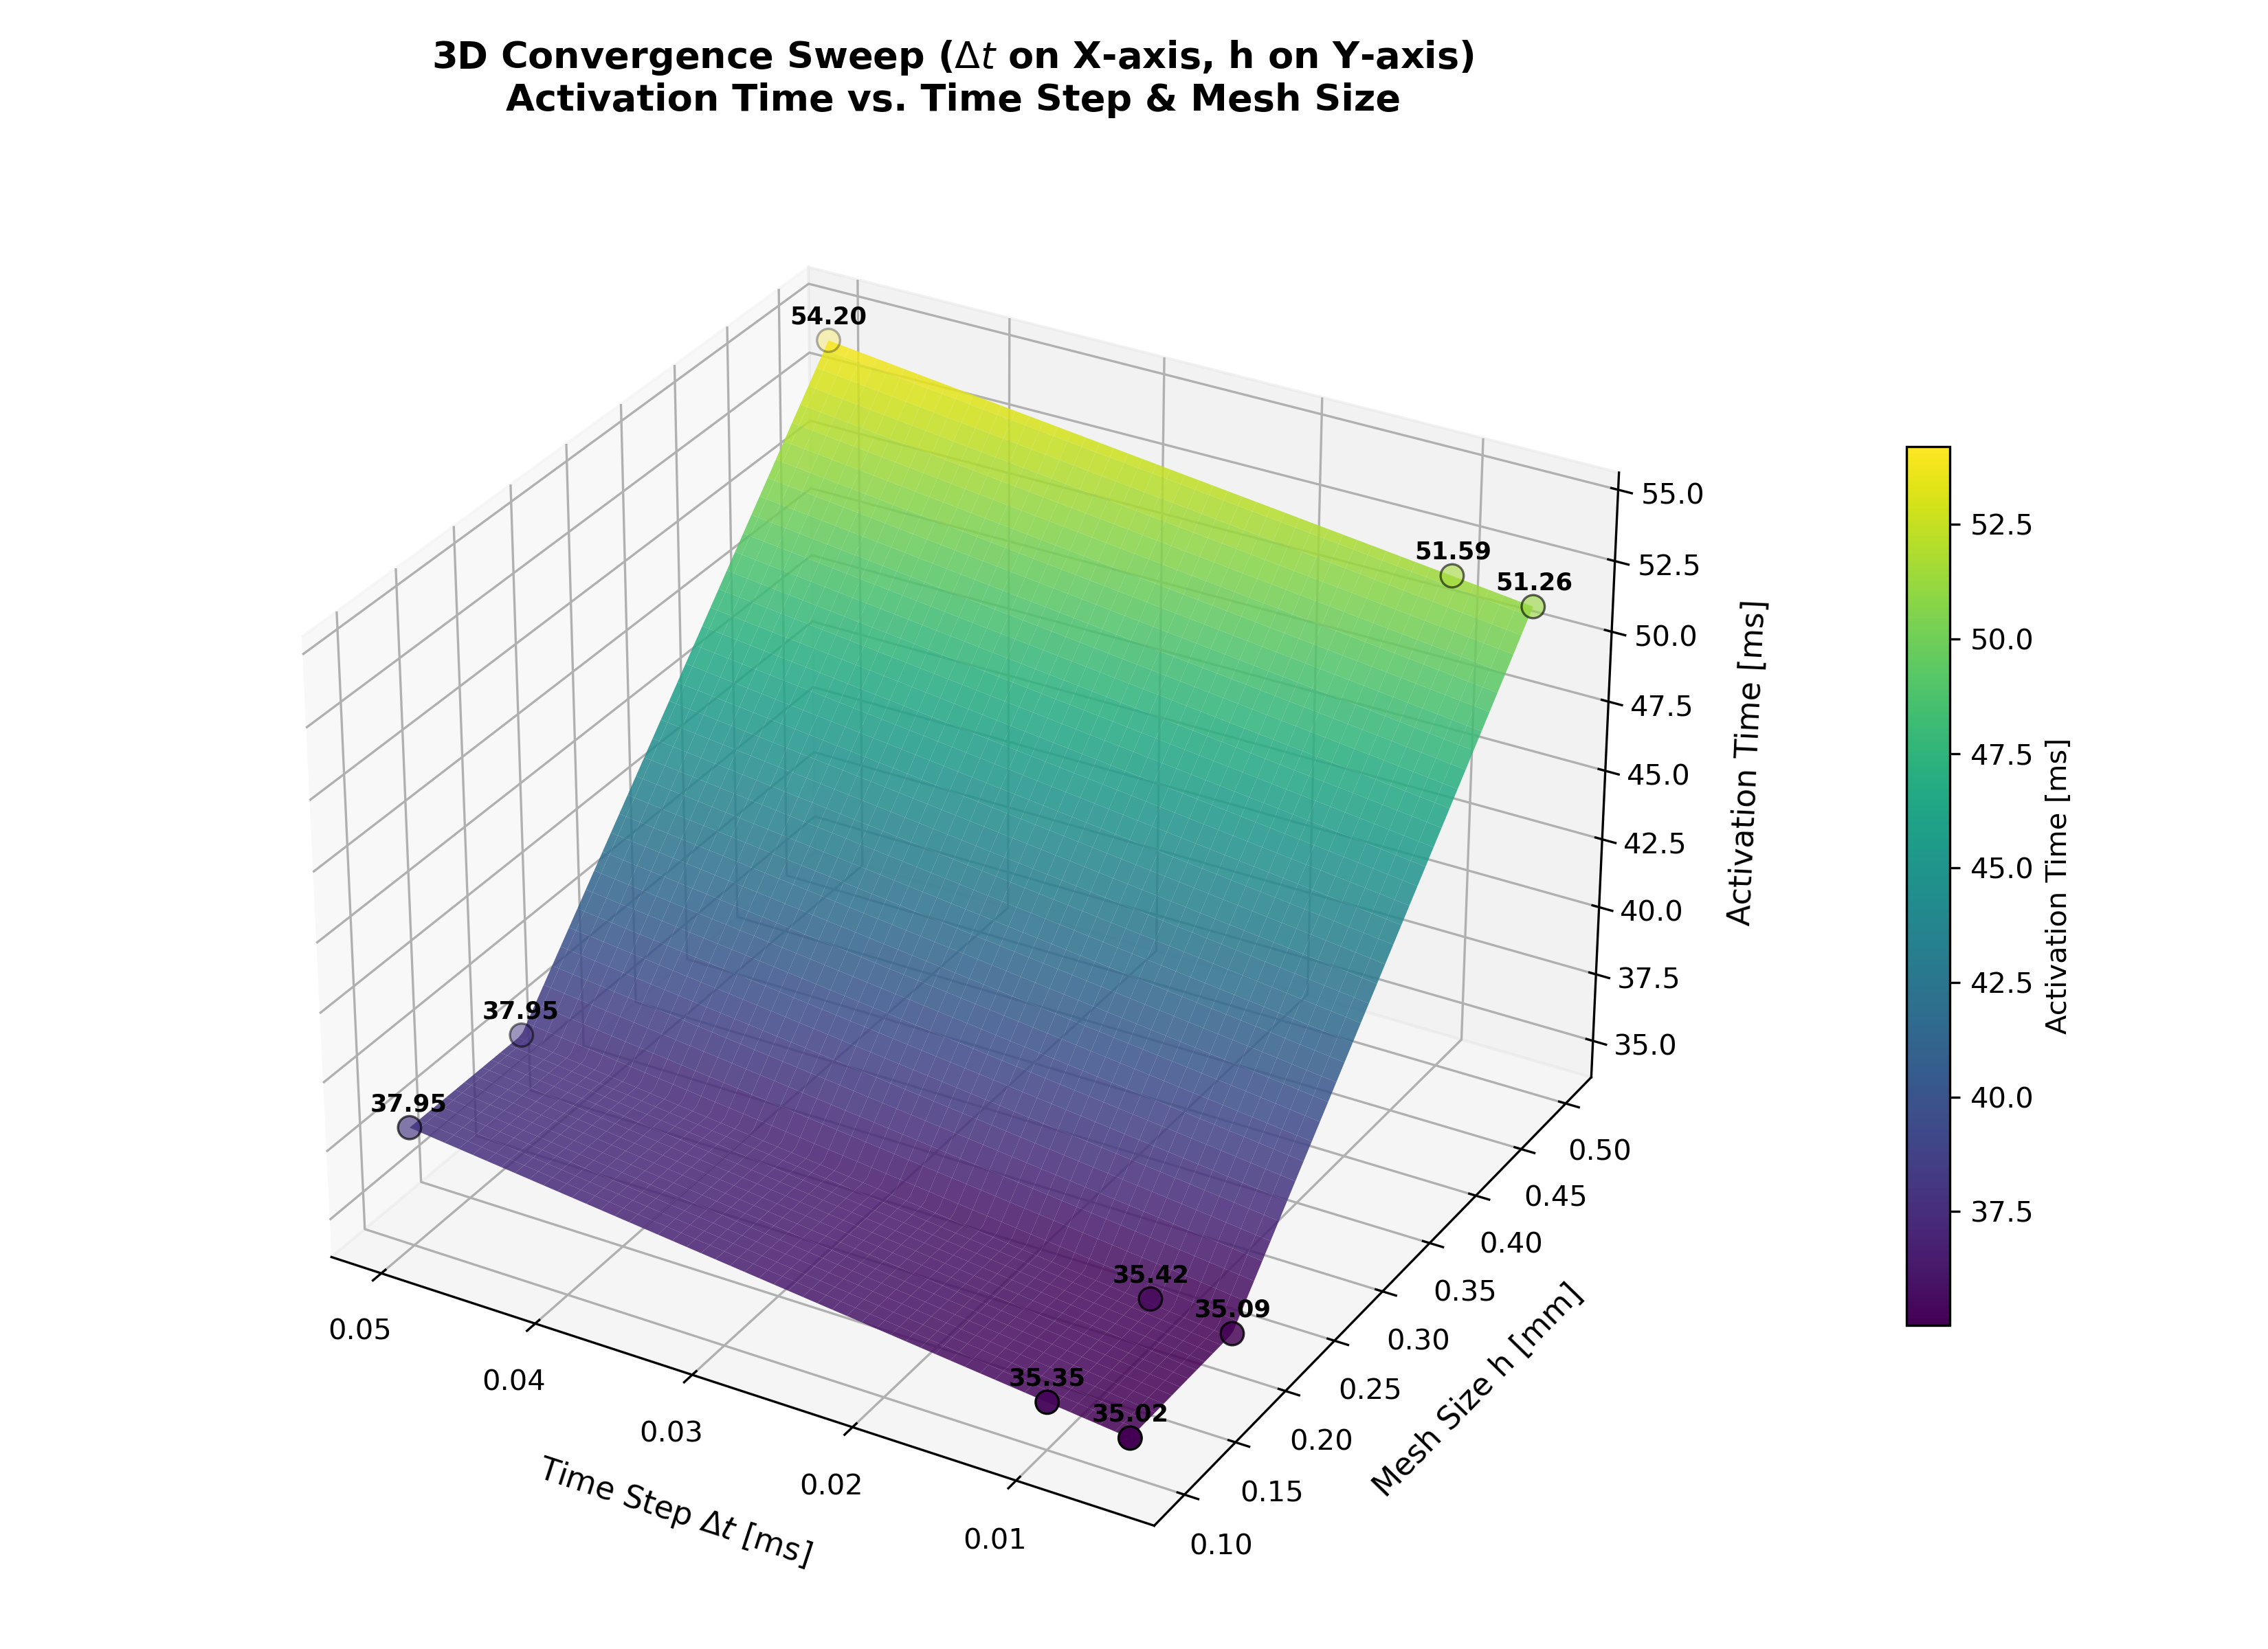
\includegraphics[width=1\linewidth]{Images/convergence_activation_time_3d.png}
    \caption{}
    \label{fig:convergence}
\end{figure}

\section{Time discretizations methods analysis}
We analyzed the influence of the time discretization scheme by parameterizing the time-stepping method with $\theta$. Specifically, we simulated the system behavior for:
\begin{itemize}
    \item $\theta = 0$ (Forward Euler);
    \item $\theta = 1$ (Backward Euler);
    \item $\theta = 0.5$ (Crank-Nicolson);
\end{itemize}
Figure~\ref{fig:euler_comparison} illustrates the activation times obtained from each method. At macroscopic scale, the resulting curves appear perfectly coincident.
\begin{figure}[H]
    \centering
    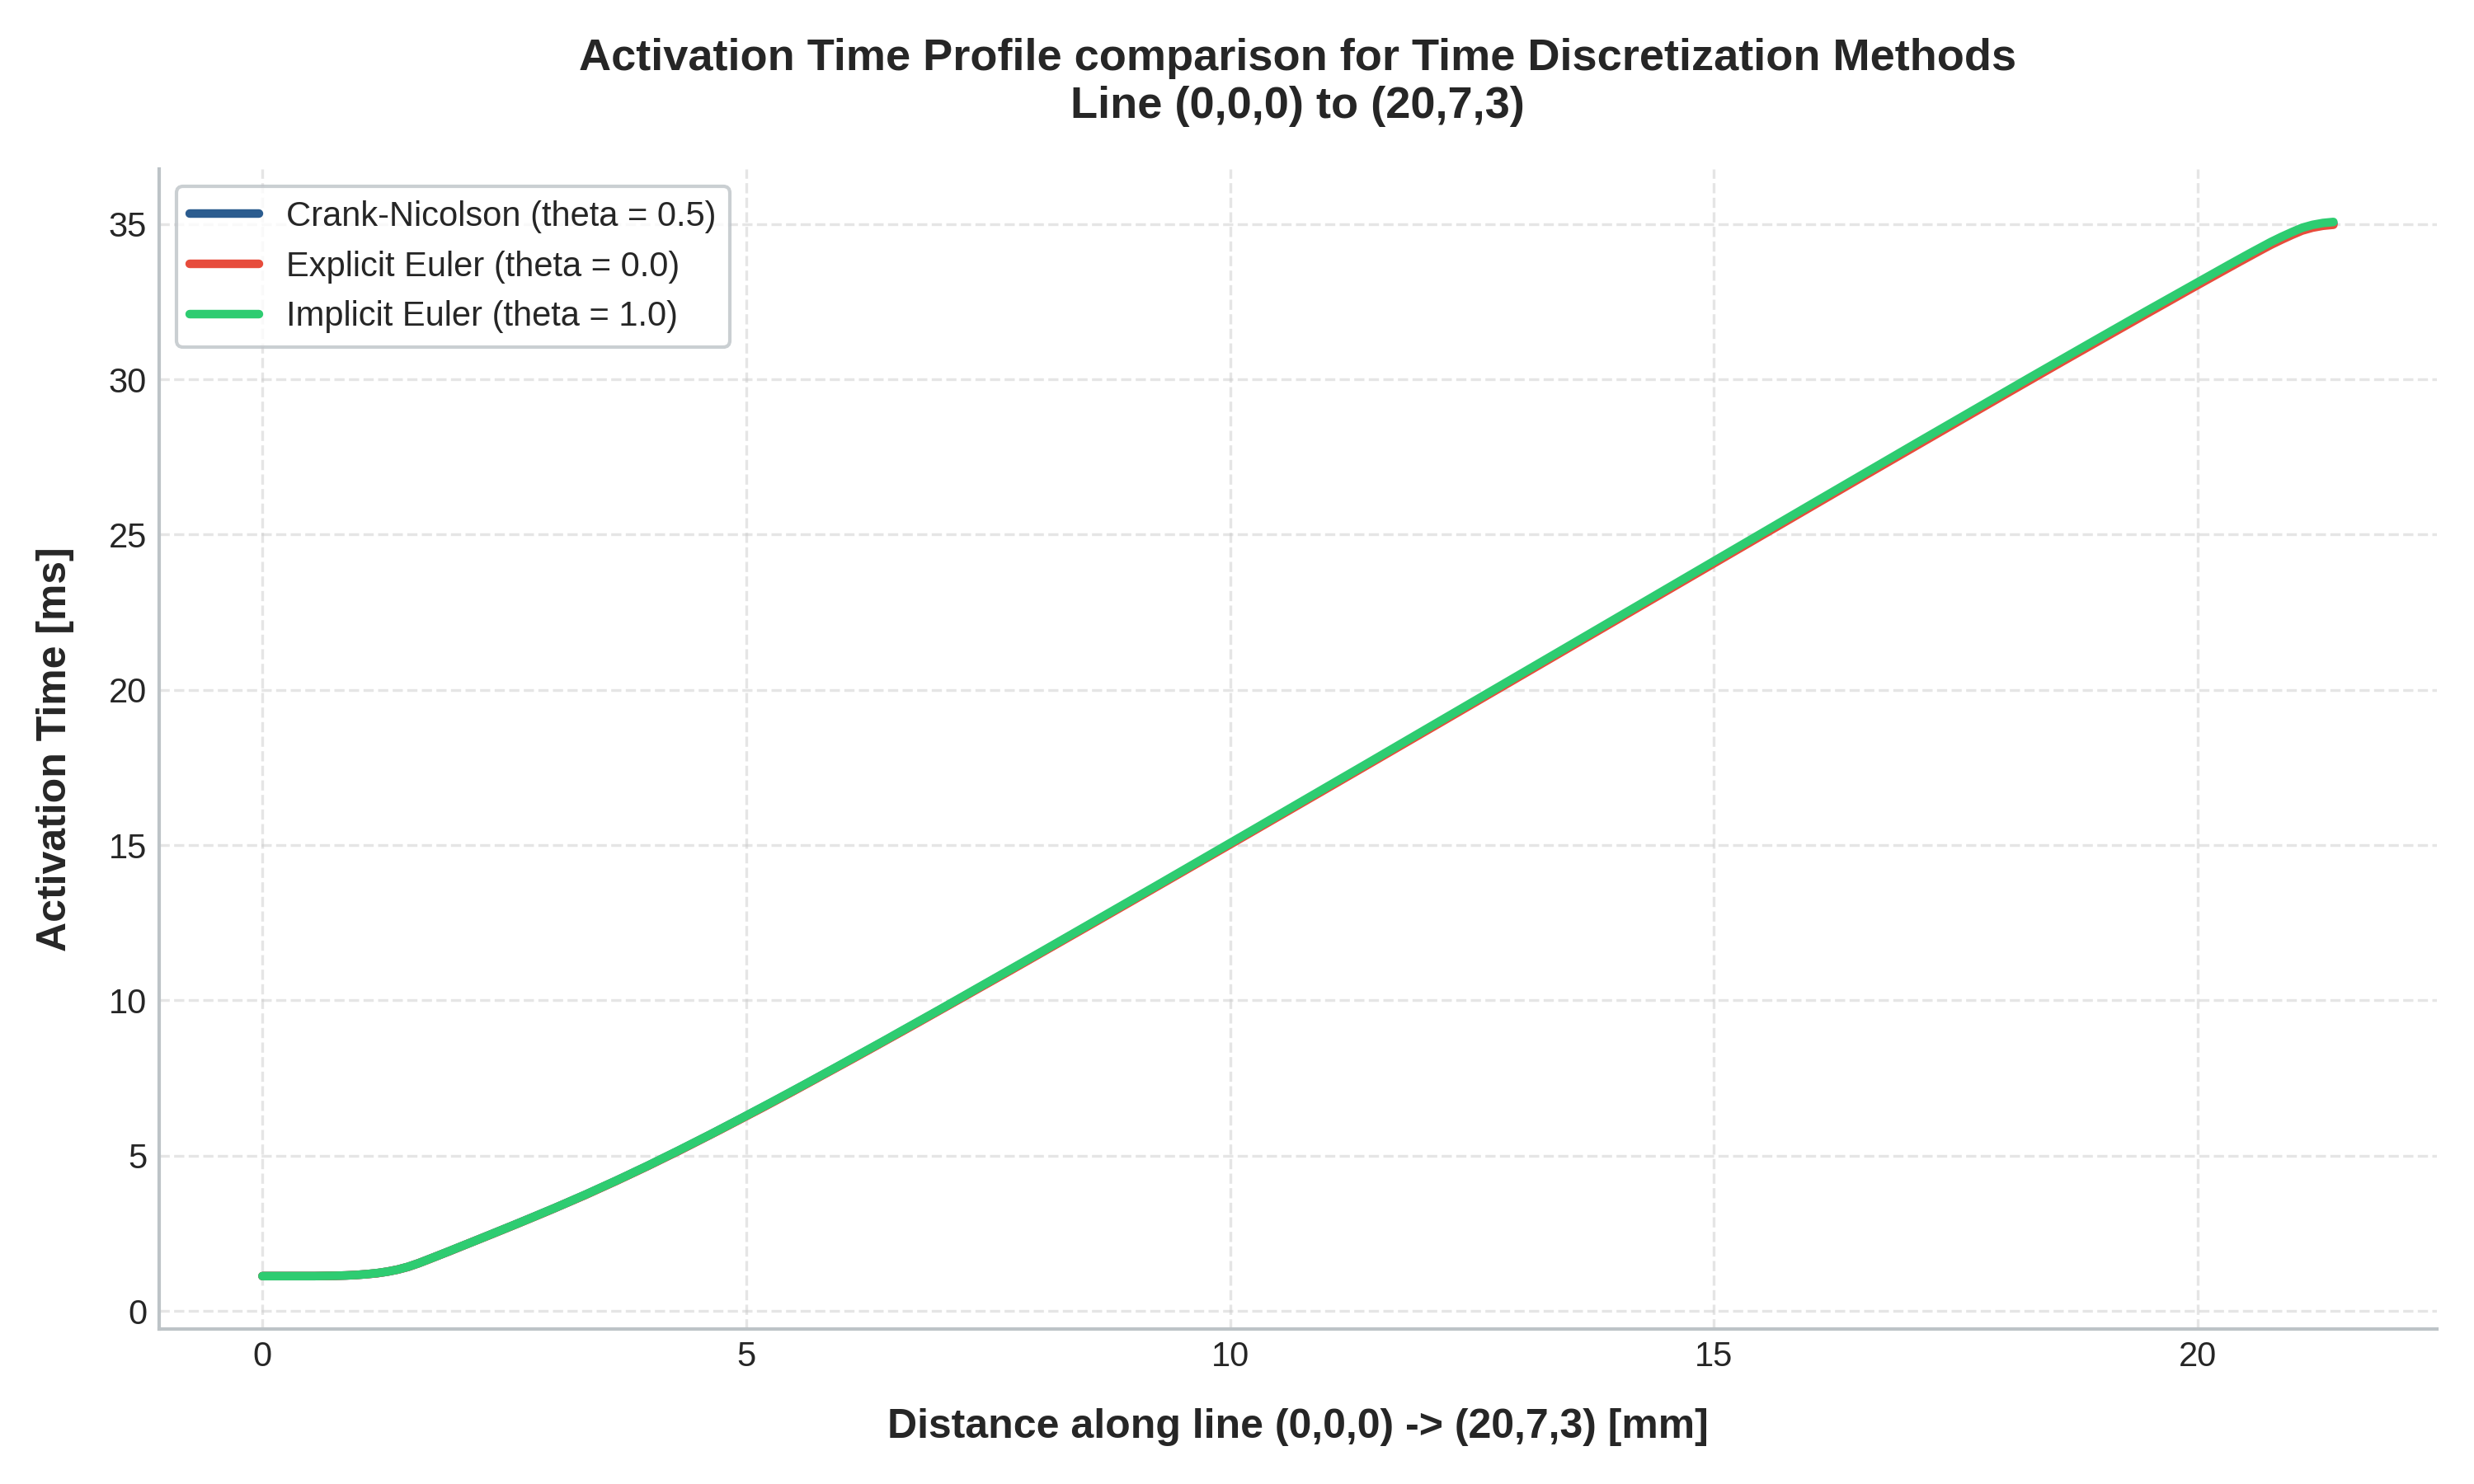
\includegraphics[width=0.75\linewidth]{Images/euler_comparison_over_line.png}
    \caption{}
    \label{fig:euler_comparison}
\end{figure}

However, a detailed inspection of the terminal phase of the simulation (Figure~\ref{fig:euler_comparison_zoom}) reveals minor discrepancies among the schemes.
The near-coincidence of the $\theta$ = 0, 0.5, 1 curves in Figs. 3.2–3.3 is the expected numerical confirmation of the analysis in Section 2.3: since the explicit forward Euler update of the gating variables is only first-order accurate by construction, it dominates the overall temporal error and fixes the convergence order of the coupled scheme to O($\Delta t$), regardless of $\theta$.

\begin{figure}[H]
    \centering
    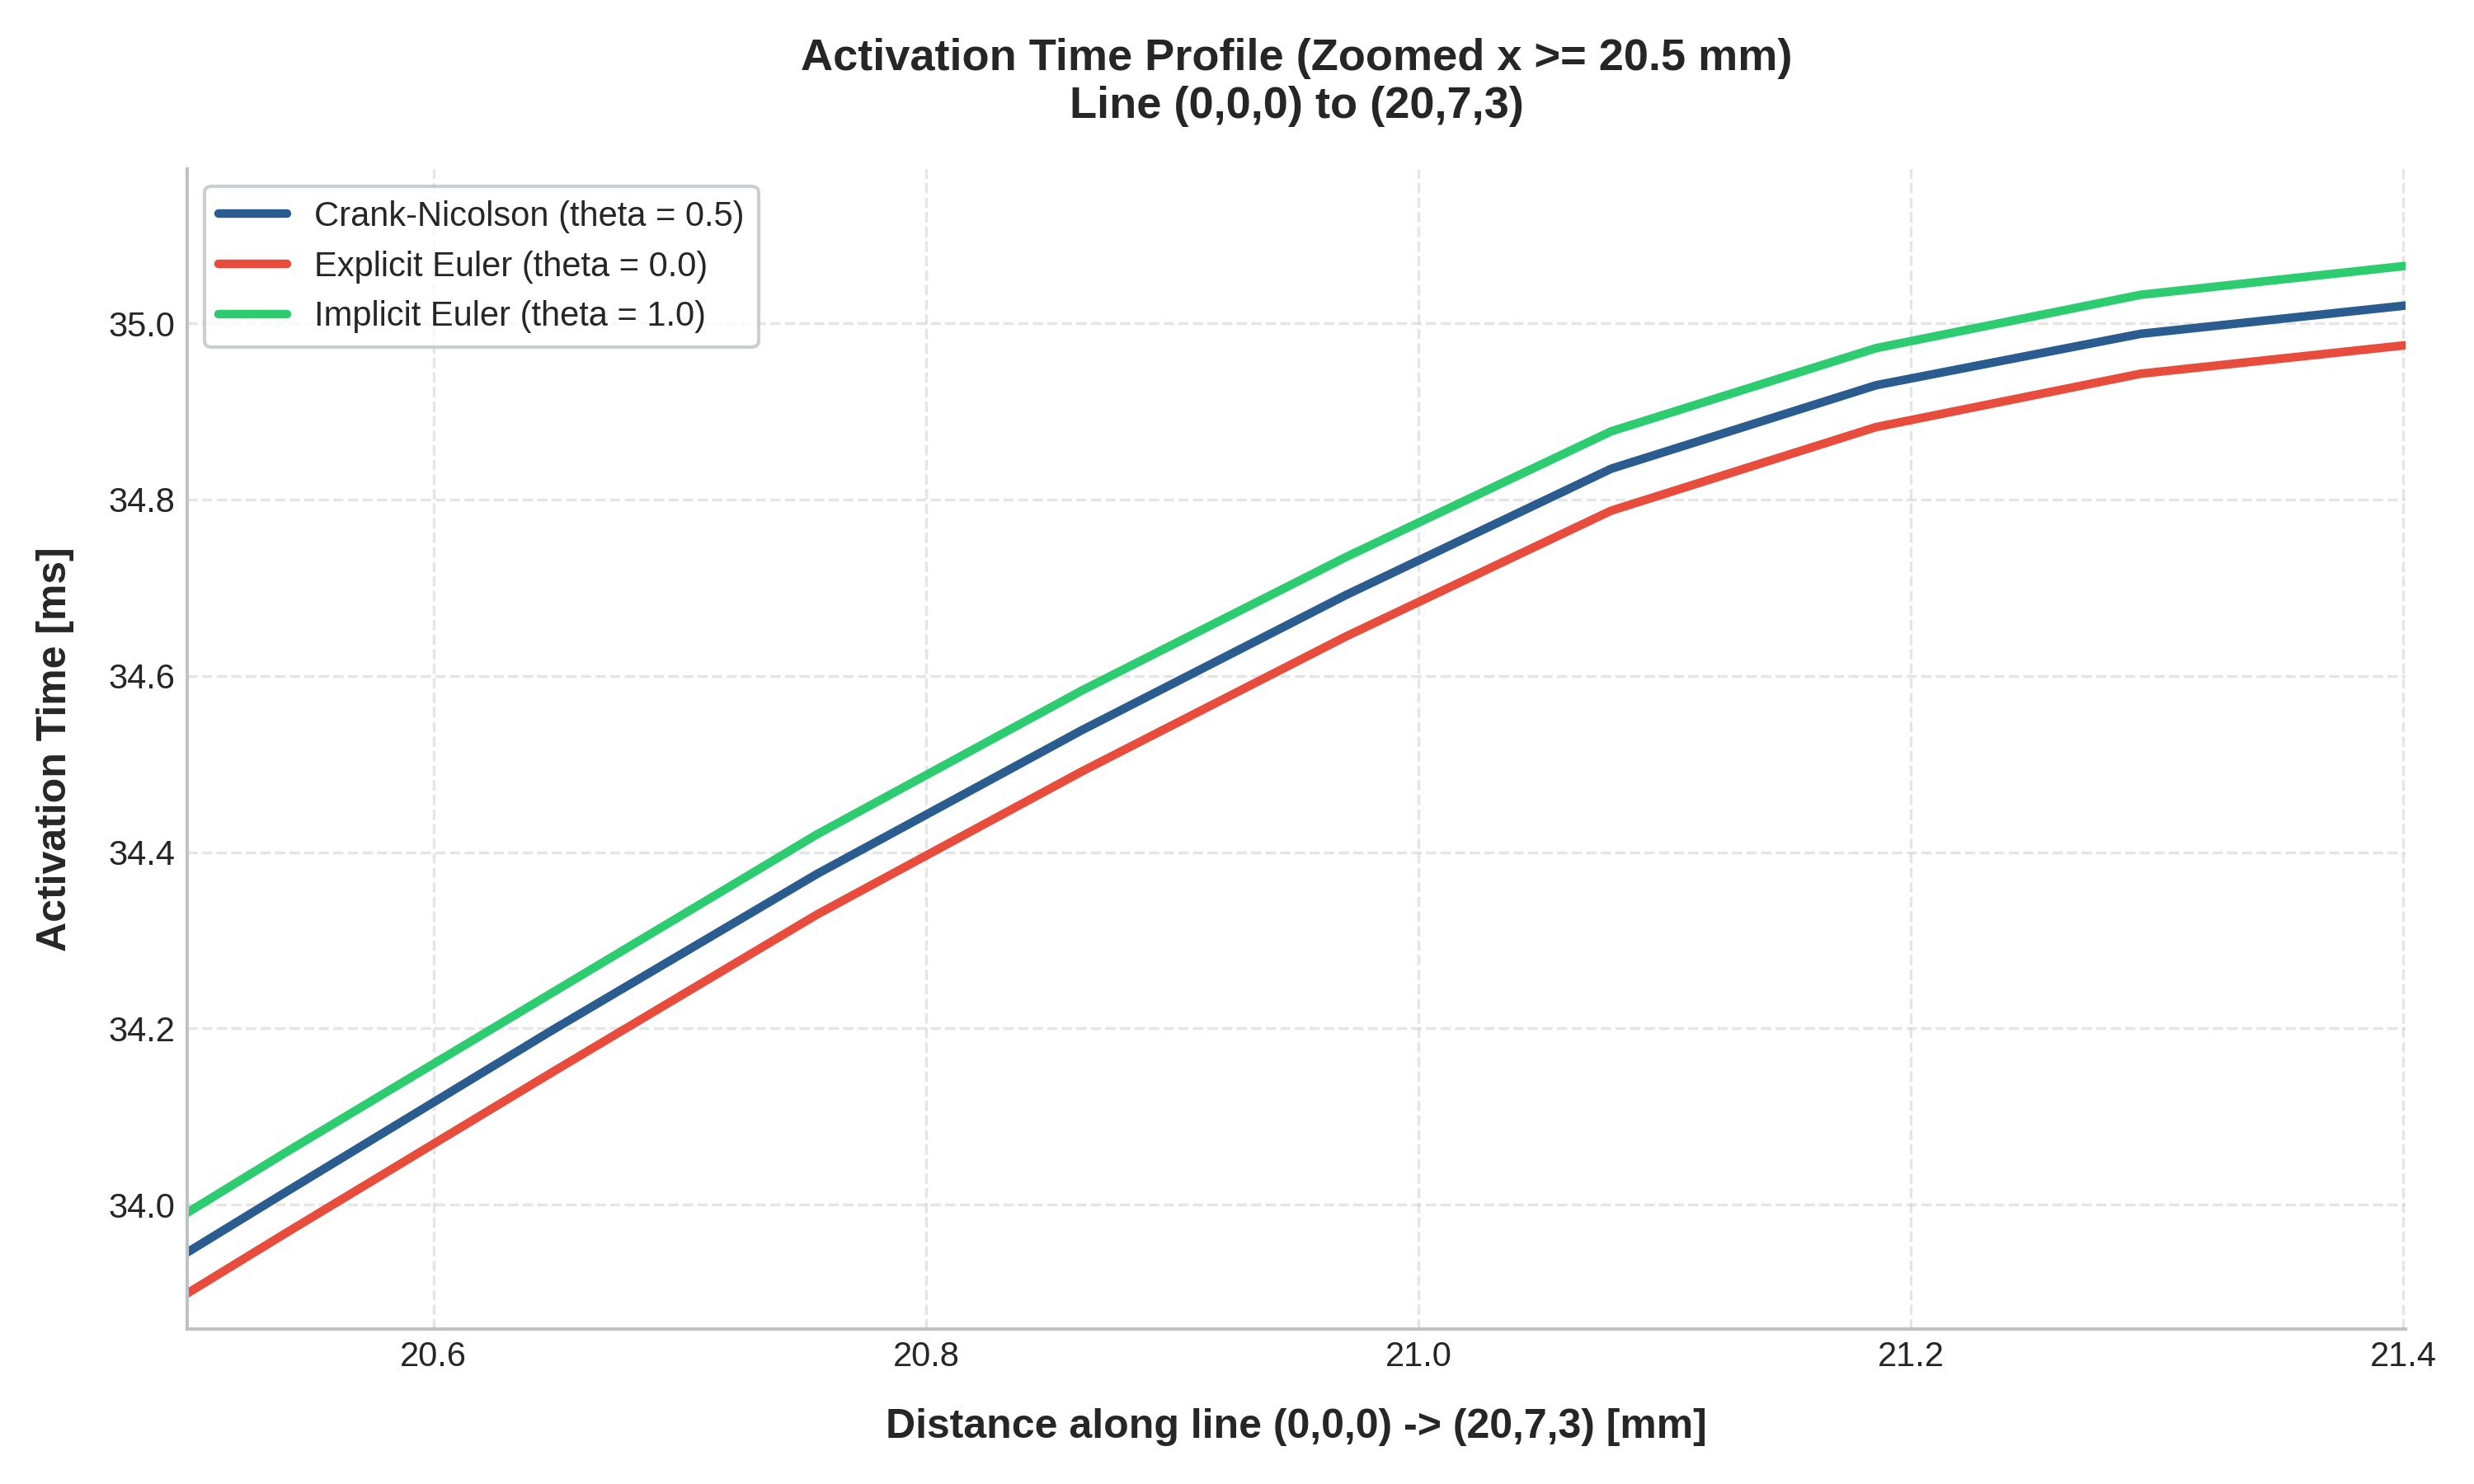
\includegraphics[width=0.75\linewidth]{Images/euler_comparison_over_line_zoom.png}
    \caption{}
    \label{fig:euler_comparison_zoom}
\end{figure}


\section{Linear solvers and preconditioners comparison}
We evaluated the performance of the numerical simulation under various solver and preconditioner configurations. Specifically, we compared the Conjugate Gradient (CG) and Generalized Minimal Residual (GMRES) iterative solvers preconditioned with Incomplete LU (ILU) factorization at different fill-in levels and Successive Over-Relaxation (SSOR). In addition, we compared these iterative approaches against a direct solver. The total execution times and average solver iterations per time step are presented in Figure~\ref{fig:solver_execution_times} and Figure~\ref{fig:solver_average_iterations}, respectively.

\begin{figure}[H]
    \centering
    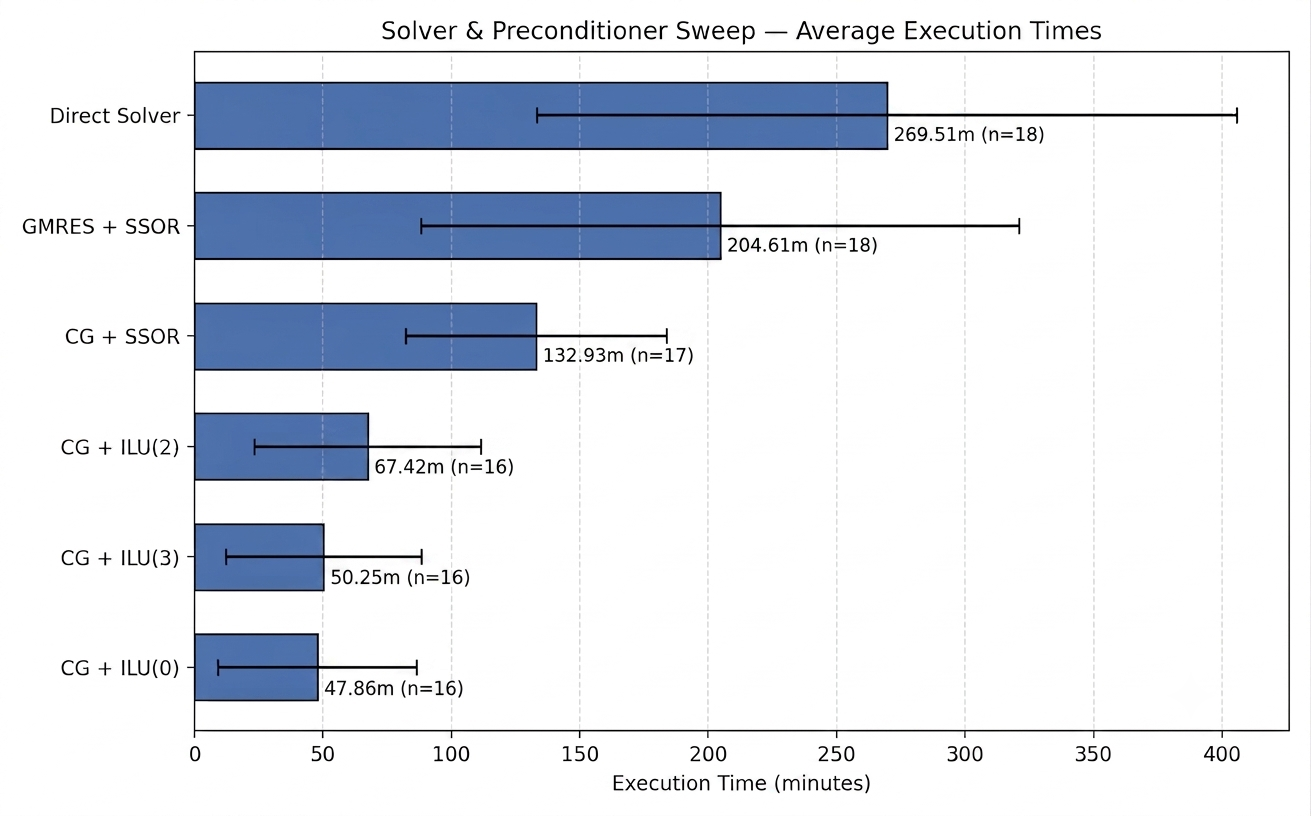
\includegraphics[width=0.75\linewidth]{Images/solver_performance_avg.png}
    \caption{Total execution times for different solver and preconditioner configurations.}
    \label{fig:solver_execution_times}
\end{figure}

The computational results reveal that the CG solver preconditioned with ILU(0) achieves the best performance, completing the simulation in average $47.86$ minutes. Increasing the fill-in level in the preconditioner does not provide a practical advantage. As shown in Figure~\ref{fig:solver_average_iterations}, the average number of iterations per time step remains virtually unchanged at $10.8$ for ILU(0), ILU(2) and ILU(3). This indicates that the cost for higher fill-in is not balanced by reduction in iteration count.

Furthermore, preconditioning with SSOR exhibits significantly worse performance due to the higher arithmetic complexity of applying SSOR in a parallel distributed-memory environment and the slightly higher average iteration counts.

\begin{figure}[H]
    \centering
    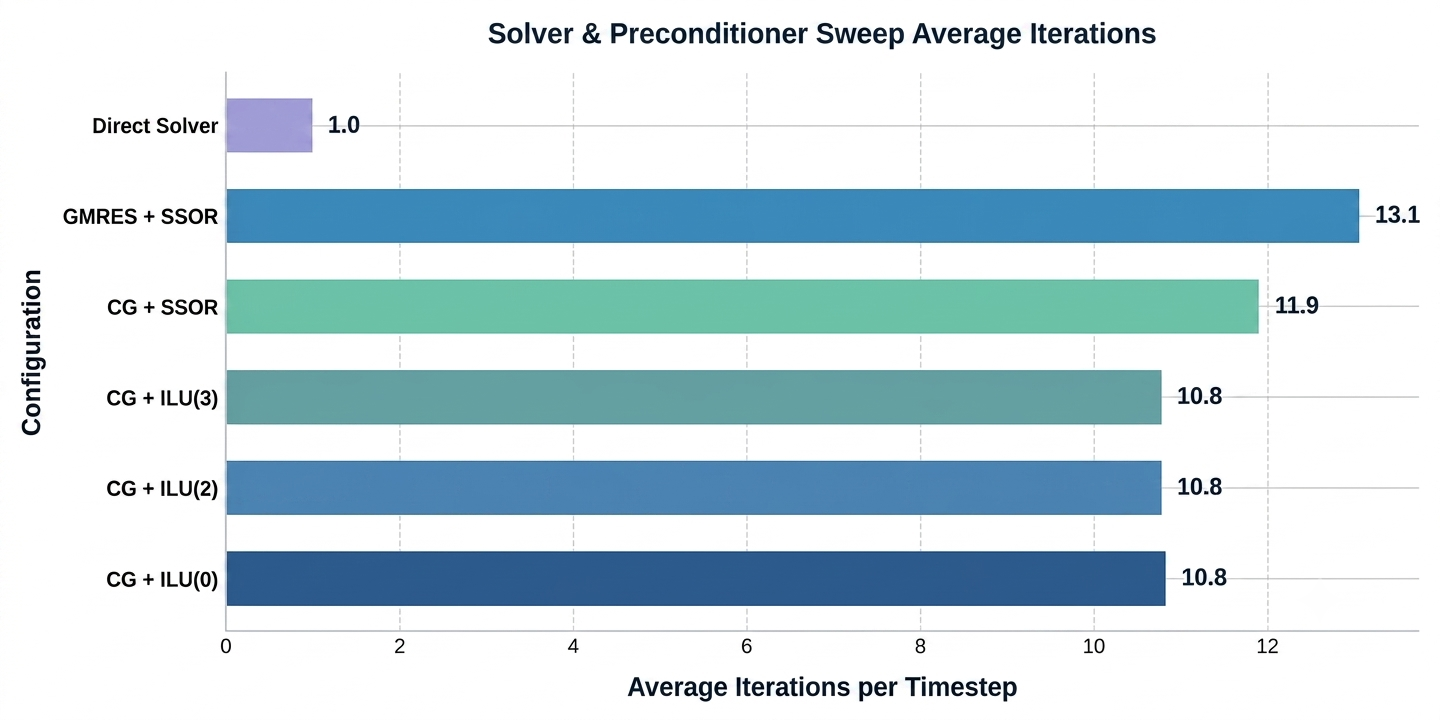
\includegraphics[width=0.75\linewidth]{Images/solver_average_iterations.png}
    \caption{Average number of solver iterations per time step for different solver and preconditioner configurations.}
    \label{fig:solver_average_iterations}
\end{figure}

Lastly, we investigated the feasibility of employing a direct solver. Because the system matrix is time-independent, its factorization can theoretically be computed once during the setup phase and reused via forward and backward substitutions to quickly solve the system at each subsequent time step. However, this approach resulted in the worst overall execution time. The system matrix, though highly sparse, is large (representing $442,401$ degrees of freedom). Direct factorization (e.g., parallel LU decomposition) suffers from severe fill-in, generating extremely dense factorization blocks. The forward and backward substitutions on these dense factors are highly memory-intensive and computationally heavy, making the direct solver impractical for large-scale cardiac simulations.
The horizontal error bars indicate the execution-time variability measured over multiple runs. These variations are mainly attributable to the inherent performance noise of the shared HPC cluster (e.g., network contention, operating system jitter, and varying system load), rather than differences in the numerical algorithms themselves.
\newpage
\section{Simulation of different parameter sets}
The developed code allows the user to select, via a
dedicated command-line option, any of the five parameter sets proposed by
Bueno-Orovio et al.: epicardial (EPI), endocardial (ENDO), midmyocardial (M),
as well as the two parameter sets designed reproduce
the dynamics of previously developed human ventricular ionic models, namely the Priebe--Beuckelmann (PB) and Ten Tusscher--Noble--Noble--
Panfilov (TNNP) models. Since all parameters governing the ionic currents and
the time constants of the gating variables are collected in a single data
structure, switching between parameter sets requires no modification to the
rest of the assembly or solution pipeline, confirming the configurability
discussed in Section 2.5.

\begin{figure}[H]
\centering

%% TOP ROW: 3 Images
\begin{subfigure}[b]{0.3\textwidth}
    \centering
    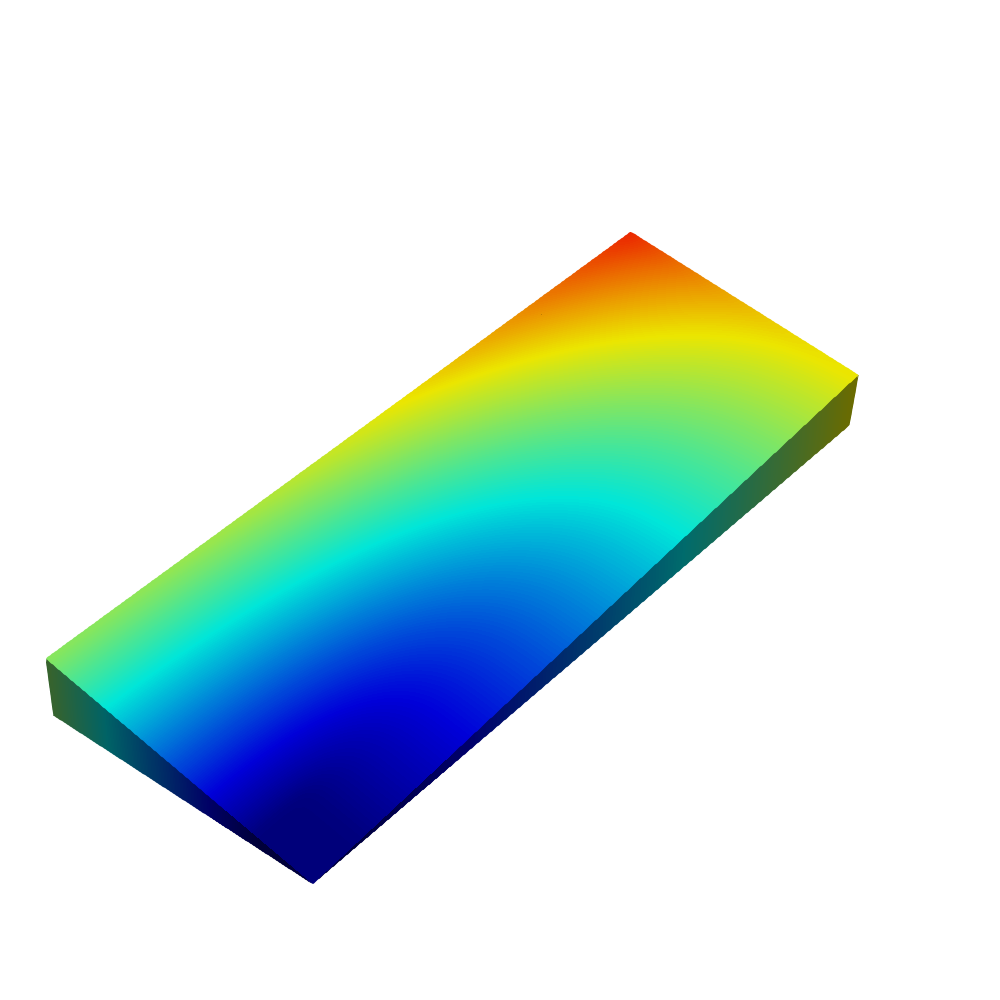
\includegraphics[width=\textwidth]{Images/EPI_activation_time_0_clip.png}
    \caption{EPI}
    \label{fig:EPI_activation_time}
\end{subfigure}
\hfill % Adds horizontal space between images
\begin{subfigure}[b]{0.3\textwidth}
    \centering
    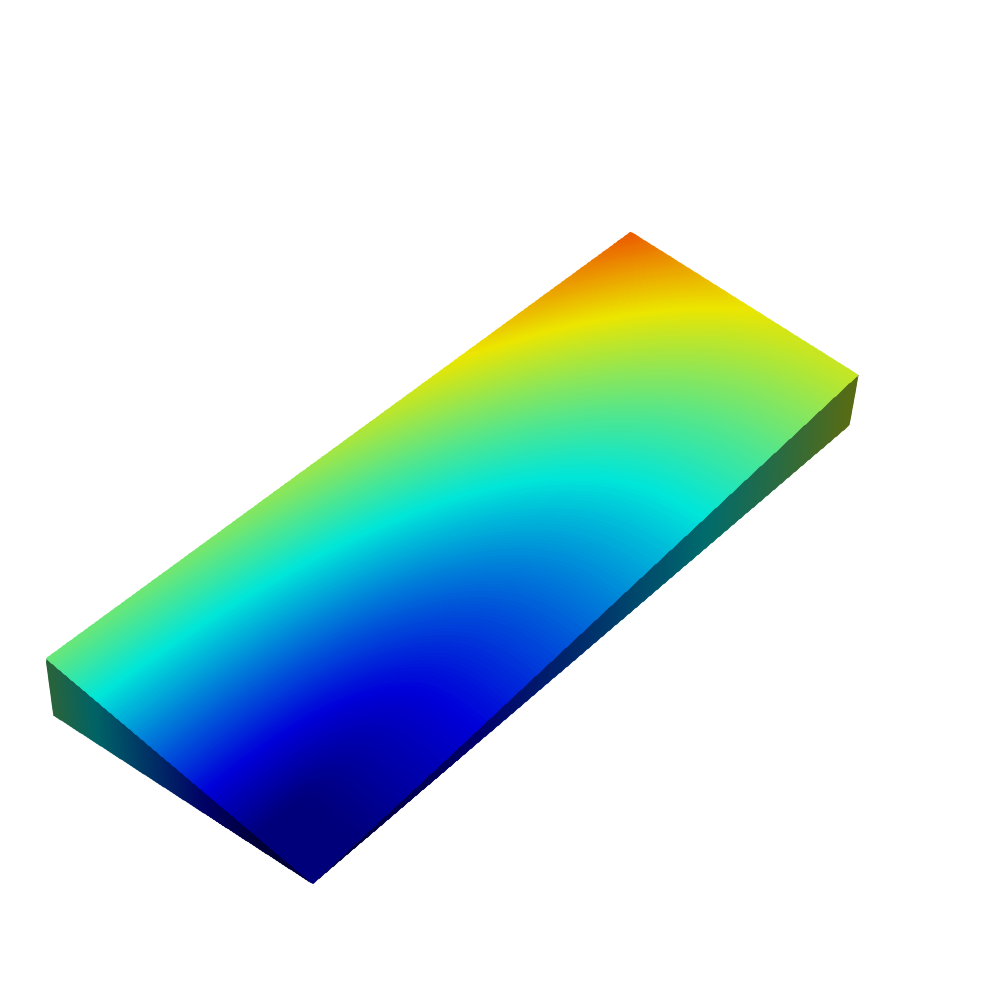
\includegraphics[width=\textwidth]{Images/ENDO_activation_time_0_clip.png}
    \caption{ENDO}
    \label{fig:ENDO_activation_time}
\end{subfigure}
\hfill
\begin{subfigure}[b]{0.3\textwidth}
    \centering
    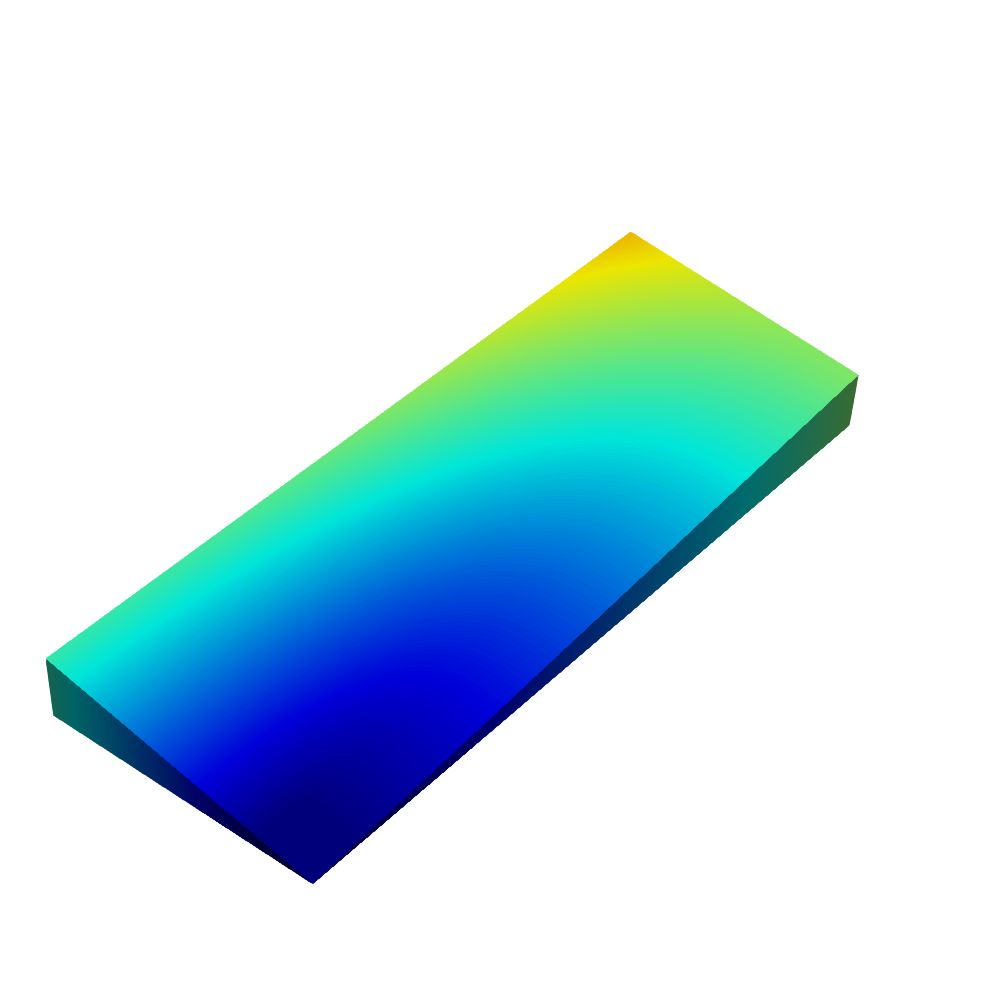
\includegraphics[width=\textwidth]{Images/M_activation_time_0_clip.png}
    \caption{M}
    \label{fig:M_activation_time}
\end{subfigure}

\vspace{0.5cm} % Adds vertical space between the two rows

%% BOTTOM ROW: 2 Images
\begin{subfigure}[b]{0.3\textwidth}
    \centering
    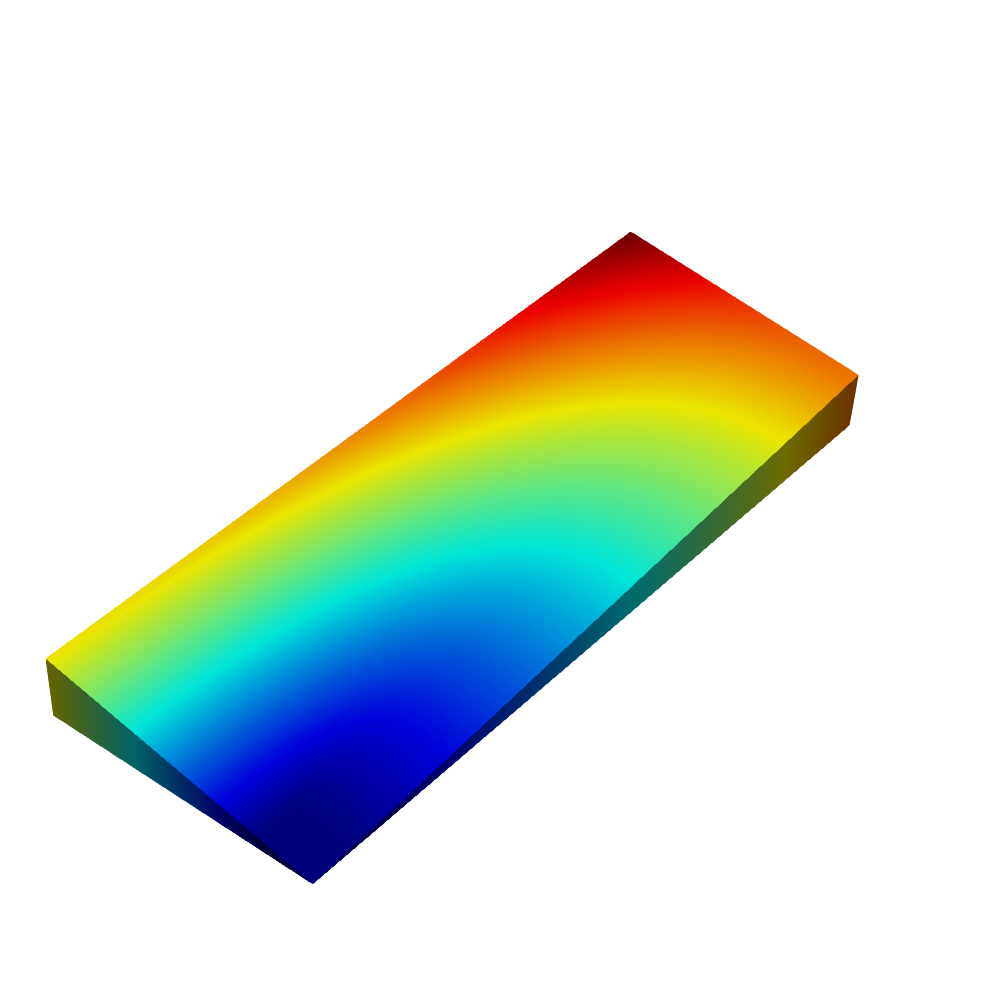
\includegraphics[width=\textwidth]{Images/PB_activation_time_0_clip.png}
    \caption{PB}
    \label{fig:PB_activation_time}
\end{subfigure}
\hfil % Using \hfil here helps center the bottom two relative to the top row
\begin{subfigure}[b]{0.3\textwidth}
    \centering
    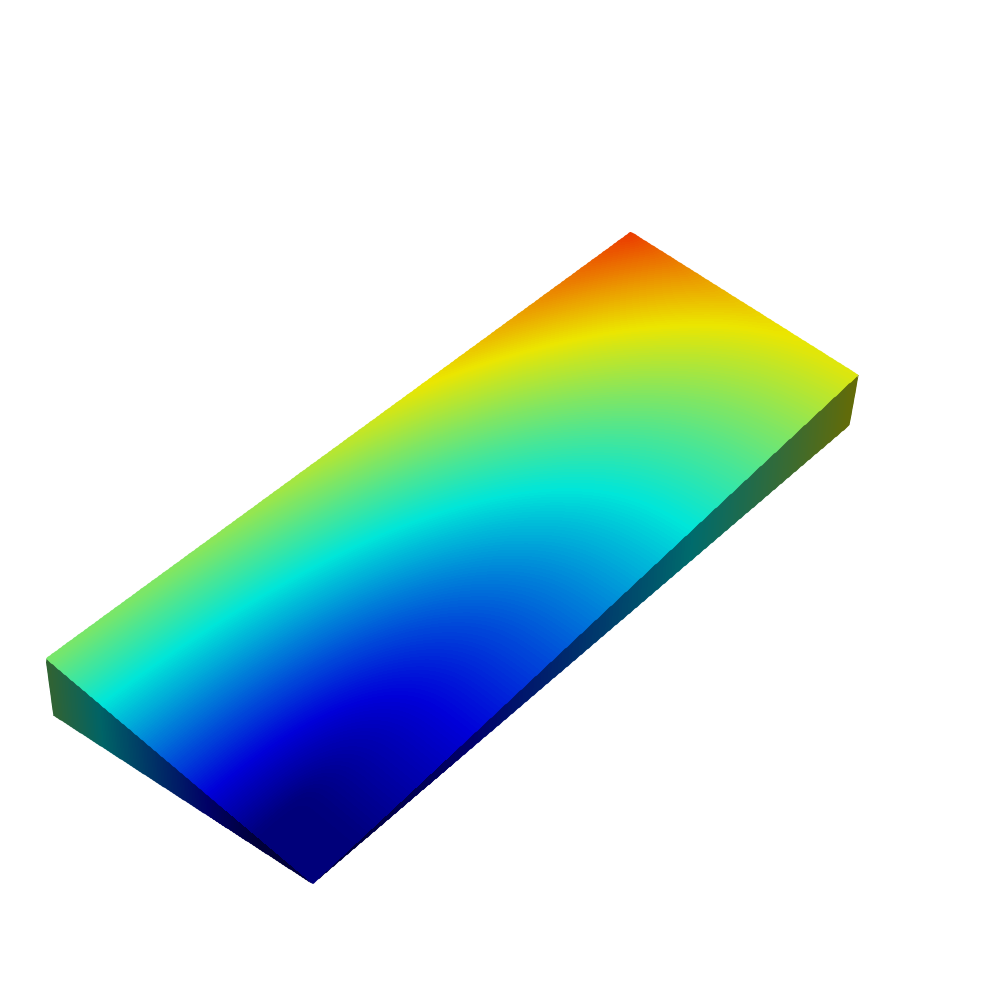
\includegraphics[width=\textwidth]{Images/TNNP_activation_time_0_clip.png}
    \caption{TNNP}
    \label{fig:TNNP_activation_time}
\end{subfigure}
\begin{subfigure}[b]{0.08\textwidth}
    \centering
    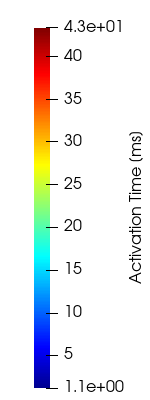
\includegraphics[width=\textwidth]{Images/colorbar_legend.png}
\end{subfigure}

\caption{}
\label{fig:models_comparison}
\end{figure}

Figure 3.6 shows the depolarization front on the same geometry (a rectangular
slab) and at the same spatial and temporal resolution for the five parameter
sets. The diffusion tensor $\Sigma$ and the domain geometry are identical in all cases.

Figure~3.7 provides a quantitative comparison of the activation time along the
diagonal of the computational domain. While all parameter sets exhibit an
approximately linear increase in activation time with distance, indicating an
almost constant propagation velocity, clear differences emerge in the slope of
the curves. The M parameter set consistently exhibits the lowest activation
times, corresponding to the fastest propagation, whereas the PB parameter set
shows the highest activation times, indicating the slowest conduction. The EPI,
ENDO and TNNP parameter sets lie between these two extremes, with EPI and ENDO
displaying very similar behaviour throughout the domain.
\begin{figure}[H]
    \centering
    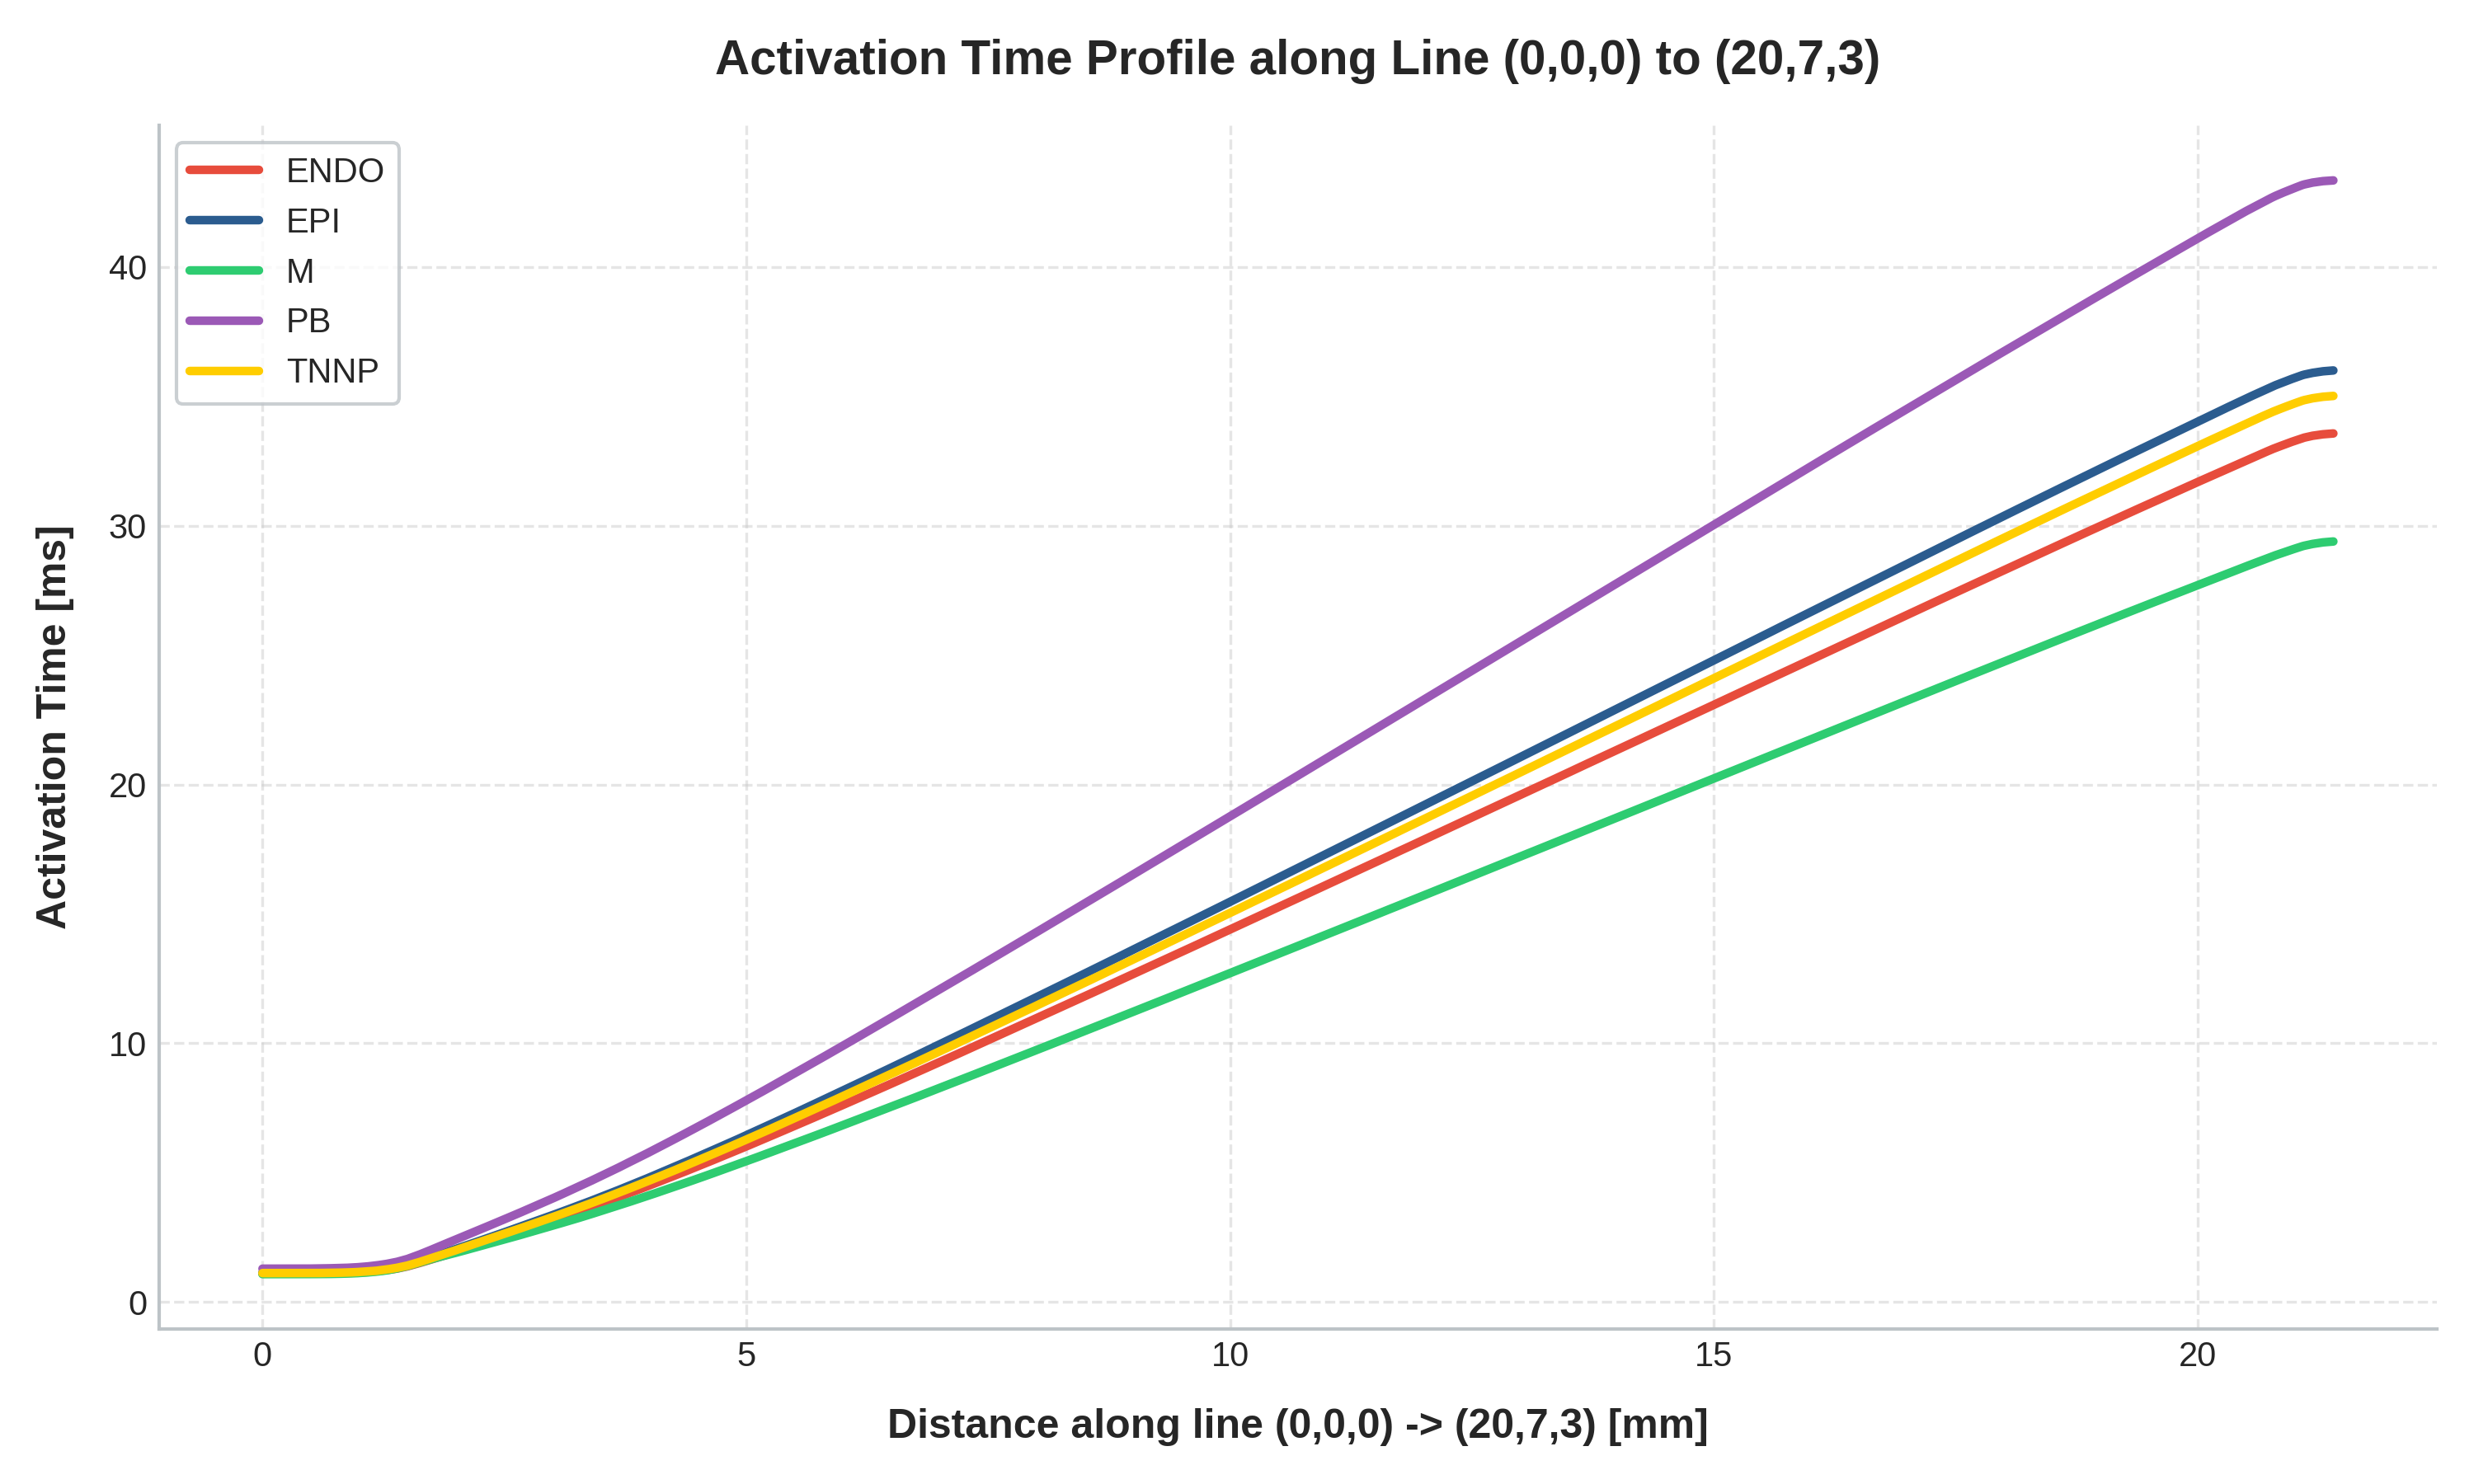
\includegraphics[width=0.75\linewidth]{Images/activation_time_over_line.png}
    \caption{Activation time over diagonal}
    \label{fig:placeholder}
\end{figure}
A zoomed view of the initial portion of the curves is provided in
Figure~3.8, highlighting the differences in the initial activation times
among the parameter sets.
\begin{figure}[H]
    \centering
    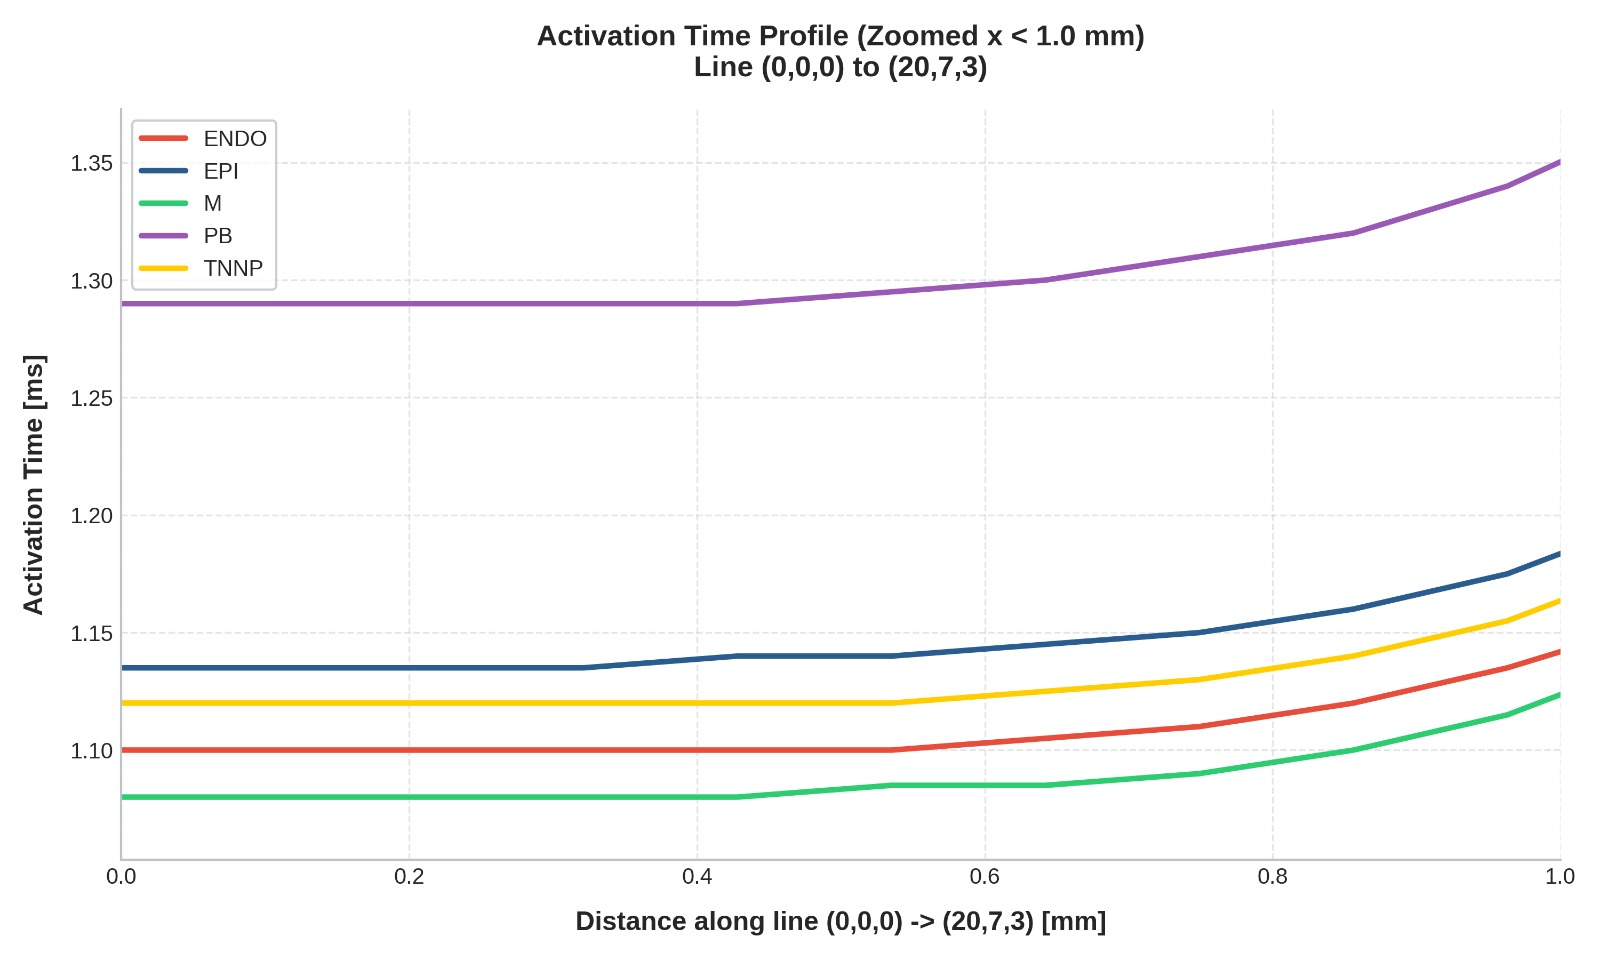
\includegraphics[width=0.75\linewidth]{Images/models_zoom.jpeg}
    \caption{Zoomed view of the initial activation time along the diagonal}
    \label{fig:placeholder}
\end{figure}
The activation time is governed exclusively by $J_{fi}$, since it is 
the first current to activate as soon as $v$ crosses $\theta_{w_1}$ 
 and the largest contributor during the upstroke, when $w_1 \approx 1$ 
and $J_{si}$, $J_{so}$ are still negligible.
\begin{table}[h]
\centering
\begin{tabular}{lcccc}
\hline
\textbf{Model} & $\tau_{fi}$ (ms) & $\theta_{w_1}$ & $v_u$ & 
\textbf{Expected CV} \\
\hline
M    & 0.078 & 0.30 & 1.61 & high \\
ENDO & 0.100 & 0.30 & 1.56 & medium     \\
EPI  & 0.110 & 0.30 & 1.55 & medium     \\
TNNP & 0.110 & 0.30 & 1.58 & medium  \\
PB   & 0.105 & 0.35 & 1.45 & low  \\
\hline
\end{tabular}
\caption{Key upstroke parameters governing the conduction velocity 
for the five Bueno-Orovio parameter sets, ordered from fastest to 
slowest wavefront propagation. $\tau_{fi}$ controls the time constant 
of the fast inward current; $\theta_{w_1}$ is the activation threshold; 
$v_u$ is the peak potential. Together they determine the amplitude of 
$J_{fi}$ (eq.~1.8) and hence the conduction velocity.}
\label{tab:upstroke_params}
\end{table}

The M model achieves the highest conduction velocity due to its smallest 
$\tau_{fi} = 0.078$~ms, which produces the strongest $J_{fi}$ and the 
steepest upstroke. The PB model is the slowest despite a $\tau_{fi}$ 
comparable to EPI and ENDO, because its higher threshold 
$\theta_{w_1} = 0.35$ and lower peak $v_u = 1.45$ jointly reduce the 
amplitude of $J_{fi}$ through the factor $(v - \theta_{w_1})(v_u - v)$ 
in eq.~1.8. EPI, ENDO and TNNP share nearly identical upstroke parameters 
and therefore produce similar activation time profiles, as confirmed by 
Figure~3.7.

This result confirms one of the main strengths of the Bueno-Orovio minimal 
model: the ability to reproduce substantially different electrophysiological 
behaviours by changing only a small number of parameters, while keeping the 
underlying numerical structure unchanged.
\section{Scalability}
Finally, the scalability analysis (Section 3.7) showed a good speed-up up to 16 MPI processes, with the execution time decreasing from 461.94 minutes (1 process) to 83.73 minutes (16 processes). Beyond this threshold, the execution time does not follow a clear monotonic trend, rising to 117.03 minutes at 32 processes but falling back to 84.95 minutes at 56 processes; given the substantial run-to-run variability observed at these process counts, this non-monotonic behaviour is likely dominated by measurement noise rather than by a clean second scaling regime. What can be stated with more confidence is that the average number of solver iterations per time step grows monotonically with the number of processes (from 3.0 to 10.8, Figure 3.10), consistent with the expected loss of effectiveness of the local ILU(0) preconditioner as the number of subdomains increases; this places an upper bound on the achievable speed-up beyond 16 processes, even if the noisy timing data do not allow a precise characterization of the trend in that regime.
\begin{figure}[H]
    \centering
    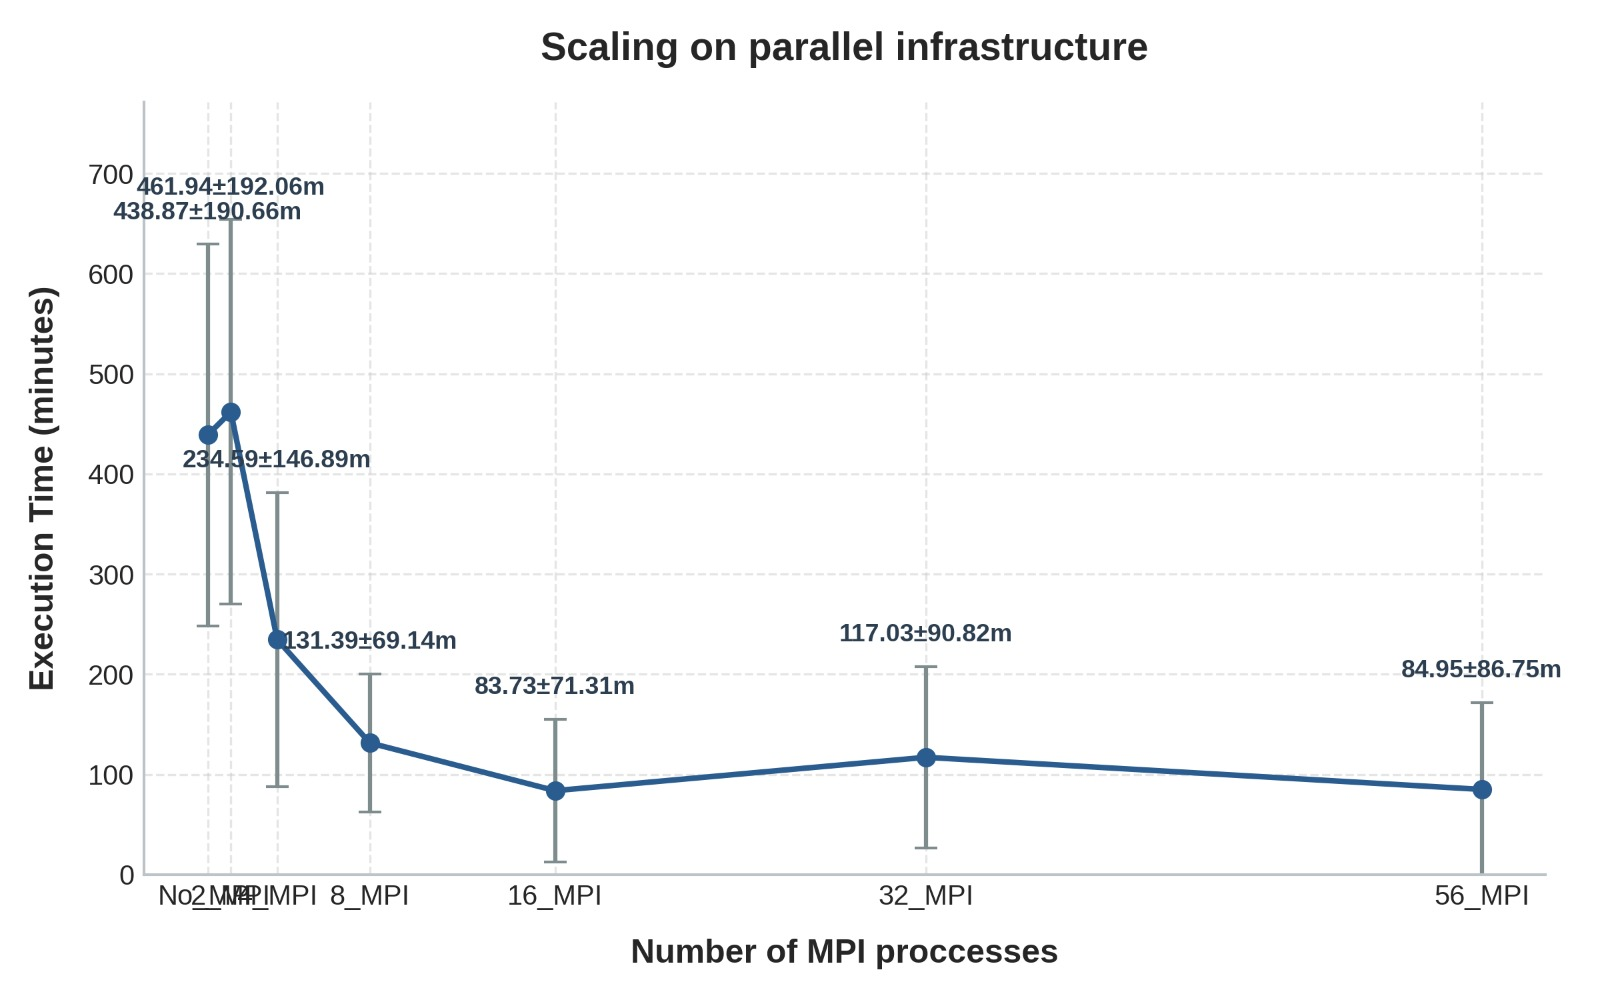
\includegraphics[width=0.9\linewidth]{Images/scalability.jpeg}
    \caption{}
    \label{fig:scalability_execution_times}
\end{figure}

\begin{figure}[H]
    \centering
    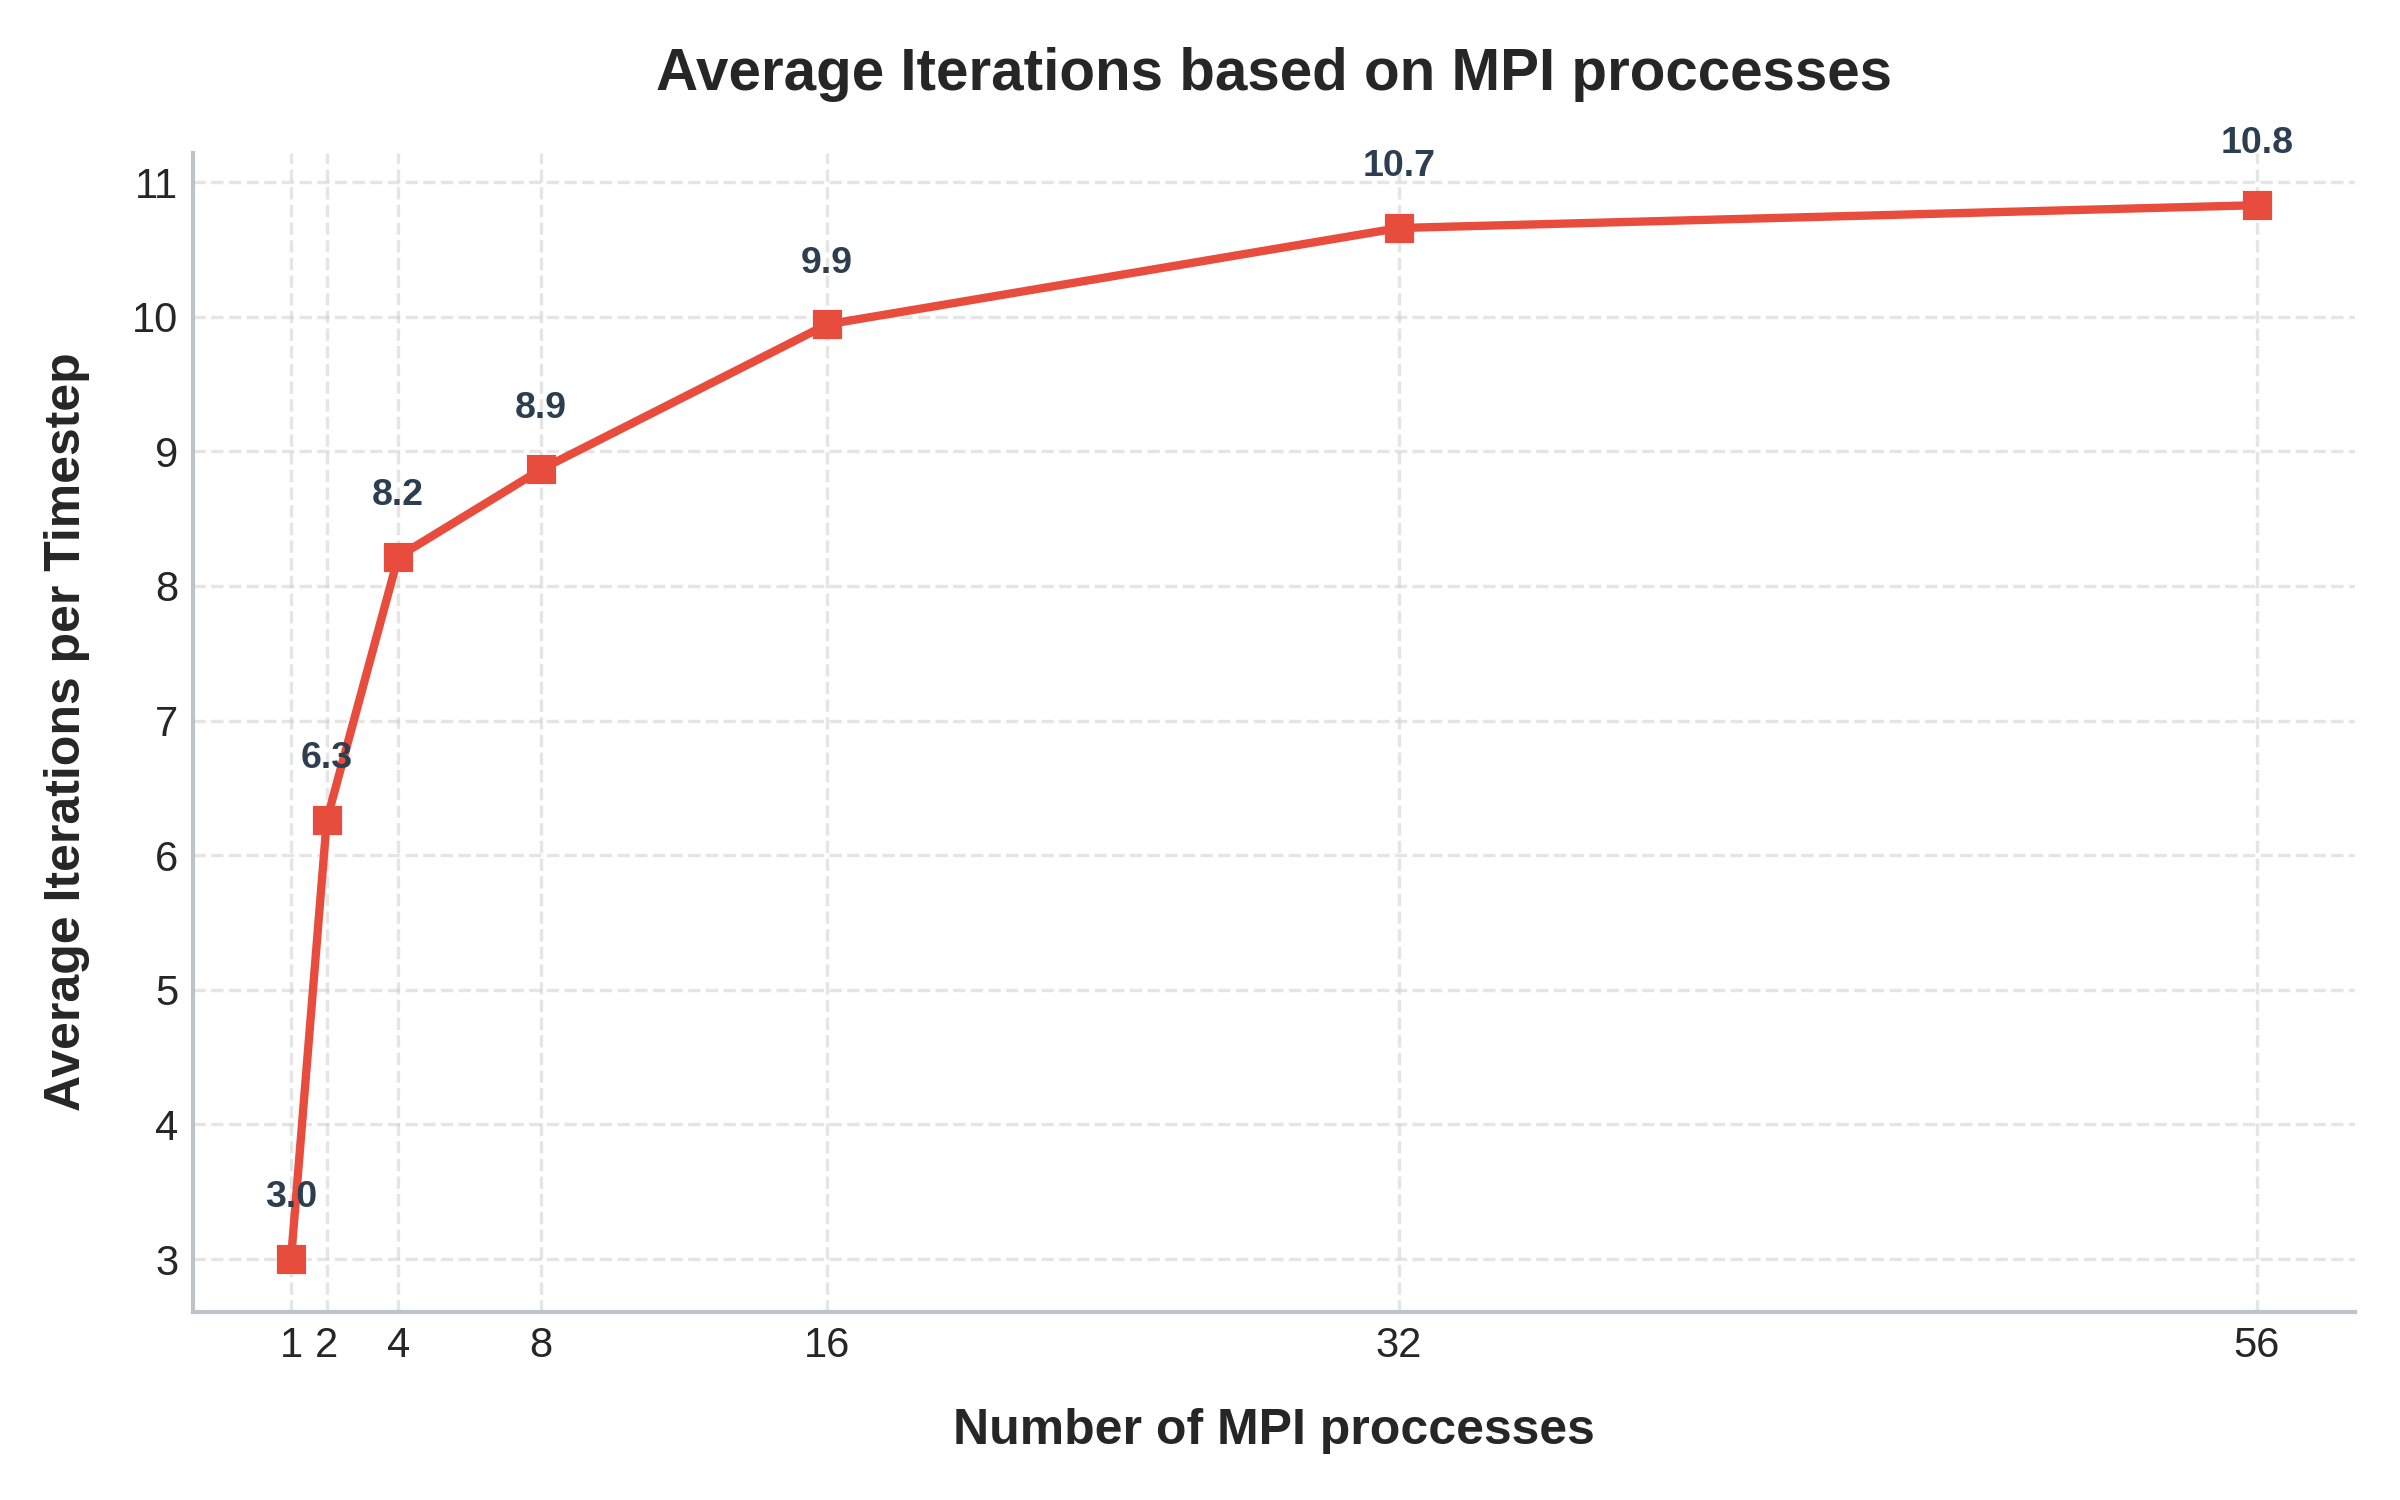
\includegraphics[width=0.75\linewidth]{Images/scalability_average_iterations.png}
    \caption{}
    \label{fig:scalability_average_iterations}
\end{figure}

\chapter{Conclusions}
In this work, a parallel solver for the monodomain model coupled with the
Bueno-Orovio minimal ionic model was implemented, based on the deal.II
library and distributed across MPI processes via the Trilinos backend. The
weak formulation and the generalized $\theta$-method time discretization,
discussed in Chapter 1, were numerically verified through a convergence
analysis with respect to the spatial step $h$ and the time step $\Delta t$
(Section 3.2), which showed the sensitivity of the activation time to both
discretization parameters, consistent with what is expected for a
reaction-diffusion problem coupled with fast gating dynamics.

The comparison between the Backward Euler, Forward Euler, and Crank-Nicolson
schemes (Section 3.3) showed that, for a fixed time step, the three
discretizations produce nearly indistinguishable solutions at the
macroscopic scale, with appreciable discrepancies only in the terminal phase
of the simulation. This result is consistent with what was discussed in
Section 2.3: the overall temporal accuracy of the scheme is in any case
limited to $O(\Delta t)$ by the explicit integration of the gating
variables, regardless of the value of $\theta$ chosen for the potential
equation alone, which explains why the differences between Crank-Nicolson
(formally $O(\Delta t^2)$) and the two Euler schemes remain small.

The comparison between linear solvers and preconditioners (Section 3.3)
showed that the Conjugate Gradient method preconditioned with ILU(0)
delivers the best performance, with a total execution time significantly
lower than both GMRES+SSOR and, especially, the direct solver, whose
inefficiency is due to the heavy fill-in generated by the factorization of a
sparse but large matrix (442,401 degrees of freedom). Increasing the fill-in
level of the ILU preconditioner does not yield significant benefits,
indicating that, for this problem, a "lightweight" preconditioner combined
with an inexpensive iterative solver represents the most efficient choice.

The extension to different cellular models (Section 3.6) confirmed the
flexibility of the Bueno-Orovio minimal model: the same numerical structure,
without any modification, reproduces both the three physiological cell
phenotypes (EPI, ENDO, M) and the parameter sets fitted to the PB and TNNP
models, showing differences in action potential morphology and conduction
consistent with those reported in the original work.

Finally, the scalability analysis (Section 3.7) showed a good speed-up up to
16 MPI processes, with the execution time decreasing from average 234.59 minutes (1
process) to average 83.73 minutes (16 processes); beyond this threshold, the
execution time increases again slightly (average 117.03 minutes at 32 processes,
average 84.95 at 56), a behaviour attributable both to the increase in the average
number of solver iterations per time step (from 3.0 to 10.8 iterations,
Figure 3.10) and to the growing weight of MPI communication relative to the
local workload as the number of degrees of freedom per process decreases.

Overall, the results obtained show that the Bueno-Orovio minimal model,
combined with a $\theta$-scheme for the diffusive part and an explicit
scheme for the gating variables, constitutes an effective trade-off between
physiological accuracy and computational cost, making it suitable for
large-scale cardiac electrophysiology simulations on HPC architectures.
Future work could focus on quantitatively validating the results against the
values reported by Bueno-Orovio and against the
verification benchmark proposed by Niederer et al., as well as on exploring
more robust preconditioning strategies to improve strong scaling beyond 16
MPI processes.

Another limitation of this work is that we were not able to perform a quantitative comparison against a fully detailed cardiac electrophysiology model. Such a comparison would have provided an additional validation of the implementation and of the numerical results. This remains an interesting direction for future work.


% @article{bueno2008minimal,
%   author  = {Bueno-Orovio, Alfonso and Cherry, Elizabeth M. and Fenton, Flavio H.},
%   title   = {A minimal model for stimulation of ventricular action potentials in human myocardium},
%   journal = {Journal of Theoretical Biology},
%   volume  = {253},
%   number  = {3},
%   pages   = {544--560},
%   year    = {2008},
%   doi     = {10.1016/j.jtbi.2008.03.029}
% }
% A. Bueno-Orovio, E. M. Cherry, and F. H. Fenton. Minimal model for human
% ventricular action potentials in tissue. Journal of Theoretical Biology, 253(3):544–
% 560, 2008.\\
% \\
% \\
% S. A. Niederer, E. Kerfoot, A. P. Benson, M. O. Bernabeu, O. Bernus, C. Bradley, E. M. Cherry, R. Clayton, F. H. Fenton, A. Garny, et al. Verification of cardiac
% tissue electrophysiology simulators using an N-version benchmark. Philosophical
% Transactions of the Royal Society A: Mathematical, Physical and Engineering Sciences,
% 369(1954):4331–4351, 2011.

\begin{thebibliography}{99}

\bibitem{buenoorovio2008}
A. Bueno-Orovio, E. M. Cherry, and F. H. Fenton. Minimal model for human ventricular action potentials in tissue. \textit{Journal of Theoretical Biology}, 253(3):544--560, 2008.

\bibitem{niederer2011}
S. A. Niederer, E. Kerfoot, A. P. Benson, M. O. Bernabeu, O. Bernus, C. Bradley, E. M. Cherry, R. Clayton, F. H. Fenton, A. Garny, et al. Verification of cardiac tissue electrophysiology simulators using an N-version benchmark. \textit{Philosophical Transactions of the Royal Society A: Mathematical, Physical and Engineering Sciences}, 369(1954):4331--4351, 2011.

\end{thebibliography}



\end{document}


